\documentclass{article}
\usepackage[margin=1in]{geometry}
\usepackage{graphicx}
\usepackage{xcolor}
\usepackage{float}
\usepackage{amsmath}
\usepackage{cite}
\usepackage{hyperref}
\graphicspath{{..} {./images}}

\definecolor{navy-blue}{rgb}{0.22,0.38,0.71}

\renewcommand{\contentsname}{\vspace*{-2\baselineskip}}

\hypersetup{
	colorlinks,
	linkcolor=black,
	urlcolor=black,
	citecolor=black
}
  		
\begin{document}
\begin{titlepage}
	\centering
	{\huge Lab 2 - Introduction to Software-Defined Radio}\\[0.25 in]
	
\includegraphics[width=0.6\textwidth]{ua_logo.png}\\[0.25 in]
	{\large \textbf{ECE 531 - Software Defined Radio\\[0.25 in]
	February 26, 2025\\[0.25 in]}}
	{\large Owen Sowatzke, osowatzke@arizona.edu\\[0.05 in]
	Department of Electrical \& Computer Engineering\\[0.05 in]
	University of Arizona, Tucson, AZ 85721\\[0.5 in]}
	\hypersetup{linkcolor=navy-blue}
	\noindent\hrulefill
	\tableofcontents
	\noindent\hrulefill
\end{titlepage}

\setlength{\parindent}{0pt}

\section{Introduction}
%Introduction to the laboratory experiment, including a brief description of the objectives and goals.

In this lab, we introduce the ADALM-PLUTO Active Learning Module (PlutoSDR). We specifically learn how to interface with the device via IIO. Then, we perform loopback collects by connecting the transmitter and receiver ports together with a coaxial cable. With the hardware in this configuration, we use MATLAB and GNU radio to perform more in-depth experiments. First, in MATLAB, we experiment with the AGC settings and determine the gain needed to saturate the receiver. Next, in GNU radio, we evaluate the parameters of the built-in PlutoSDR blocks and once again determine the gain needed to saturate the receiver. We also observe the frequency response and learn how to map the input frequency to the RF frequency. Next, we create our own PlutoSDR blocks from IIO primitives and validate the behavior of these blocks. Finally, we use MATLAB to measure the SNR of the received signal for different gain levels and AGC settings. 

\section{Procedure}
% Detailed explanation of the laboratory experiment, including the design, implementation, and testing of the system.

In this section, we outline the procedures for each of our experiments. We start by interfacing with the device via IIO. Then, we perform loopback collects in MATLAB and GNU Radio. For our GNU radio experiments, we perform the outlined procedure with the default PlutoSDR blocks and generic IIO blocks. Finally, we present a method for measuring the SNR.

\subsection{Industrial Input/Output (IIO)}
\label{section::industrial_input_output}

In this experiment, we learn how to interface with the PlutoSDR with IIO. We start by executing the \texttt{iio\_info -s} command to identify the PlutoSDR device's Universal Resource Identifier (URI). We perform this step in an SSH terminal session connected to the embedded PlutoSDR operating system and in a local PC terminal. Then, we compare the resulting URIs. Next, in the SSH terminal, we use the \texttt{iio\_attr} command to locate the \textit{ad9361-phy} device. Once we find the device, we use the following command to verify its name:

\begin{center}
\texttt{cat /sys/bus/iio/devices/$<$iio\_device$>$/name}
\end{center}

where \texttt{$<$iio\_device$>$} is the IIO device we found with the \texttt{iio\_attr -s} command. Finally, we use the \texttt{iio\_attr} command to list the attributes of the \textit{ad9361-phy} device.

\subsection{MATLAB Loopback}

In this experiment, we perform a loopback test by connecting the Pluto SDR's transmit and receive ports together with a coaxial SMA cable. Once the cable is properly connected, we execute the provided \texttt{loopback.m} script to perform a physical collect. After validating that our loopback collect works, we evaluate the impact of the \textit{GainSource} (AGC) settings by testing each of its possible configurations: \textit{Manual}, \textit{AGC Slow Attack}, and \textit{AGC Fast Attack}. To characterize the impact of these settings, we modify our transmitted signal by adding segments of zeros. Finally, we determine what gain values are necessary to turn the receive sinusoid into a square wave (saturate the signal).

\subsection{GNU Radio Loopback}
\label{section::gnu_radio_loopback}

We can perform a similar loopback experiment using GNU Radio instead of MATLAB. For this test, we use the provided \texttt{PlutoTestSine.grc} flowchart. The lab assignment also mentions a ``QT GUI Time Sink", which is not included in the provided flowchart. To meet the requirements of this experiment, we have added the time sink to the flowchart. The resulting flowchart is shown in Figure \ref{fig::gnu_radio_loopback_flowchart}.

\begin{figure}[H]
	\centerline{\fbox{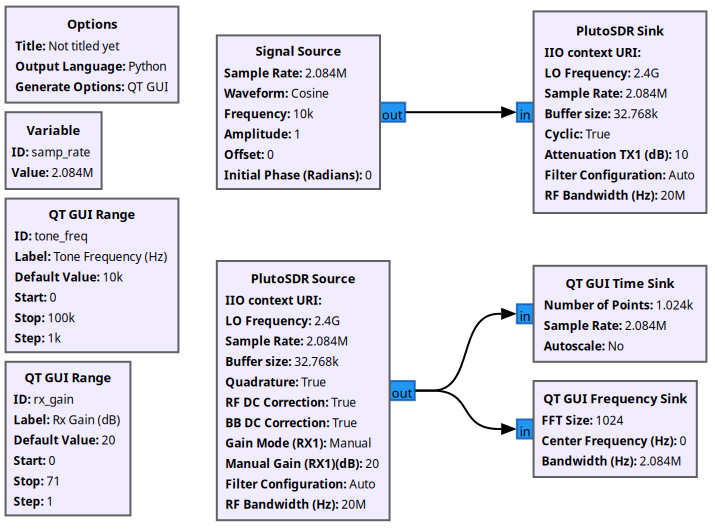
\includegraphics[width=0.5\textwidth]{gnu_radio_loopback_flowchart.png}}}
	\caption{GNU Radio Flowchart for Loopback Test}
	\label{fig::gnu_radio_loopback_flowchart}
\end{figure}

Before we run the flowchart, we review the properties of the PlutoSDR blocks. We specifically investigate the RF bandwidth and its impact on performance. Then, we describe what the ``Cyclic" option does in the PlutoSDR sink. Finally, we discuss the effects of Manual Gain control in the Pluto SDR and review alternative gain control strategies.

After reviewing the PlutoSDR blocks, we run the flowchart and determine the receiver gain where the signal distorts (or clips). Next, we replace the ``QT Time Sink" and ``QT Frequency Sink" blocks with a ``QT GUI Sink" block. Using the updated flowchart, we examine the impacts of increasing the number of averages and changing the window function. Then, we determine the transmitted RF frequency and explain how our transmitter configuration results in this frequency.

\subsection{GNU Radio as a libIIO Client}

For this experiment, we replace the PlutoSDR source and sink blocks with generic IIO blocks. The generic IIO blocks and their default values are given in Figure \ref{fig::generic_iio_blocks}.

\begin{figure}[H]
	\centerline{\fbox{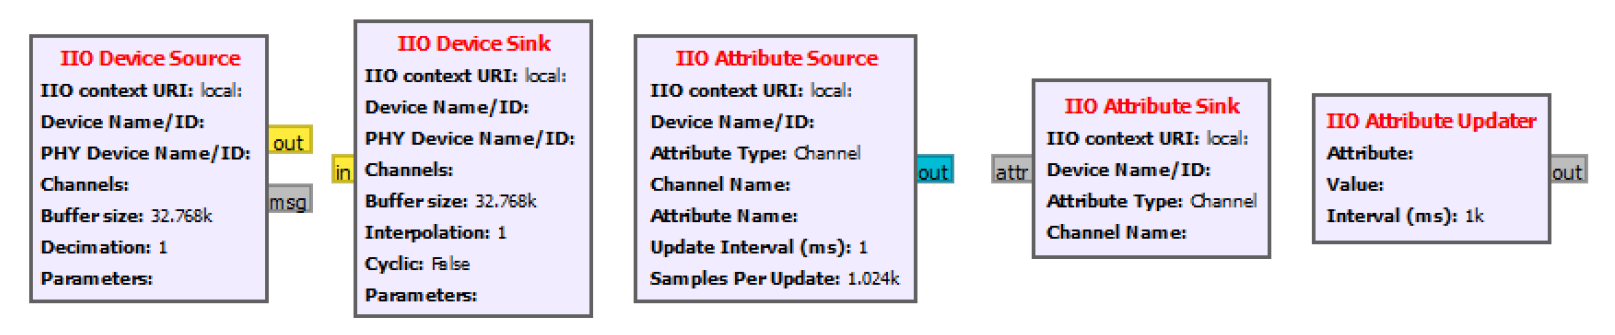
\includegraphics[width=0.8\textwidth]{generic_iio_blocks.png}}}
	\caption{Generic IIO Blocks with Default Values}
	\label{fig::generic_iio_blocks}
\end{figure}

After replacing the PlutoSDR source and sink blocks with the blocks shown in Figure \ref{fig::generic_iio_blocks}, we repeat the experiment from Section \ref{section::gnu_radio_loopback}. Then, we change the transmit and receive LO frequencies from 2.4 GHz to 915 MHz and increase the sampling rates from 2.084 MSPS to 4 MSPS. Finally, we verify that each of these settings are correctly applied using the \texttt{iio\_attr} command. 

\subsection{Measurements and the Radio}
\label{section::snr_measurement}

In this experiment, we use measure the SNR of the Pluto loopback signal with MATLAB. We collect data with a 50\% duty cycle. Then, we use the "zero" regions of the received signal to measure the noise power and the portions of the signal with the sinusoid to measure the power of the signal plus noise. With our measurements, we estimate the signal to noise ratio as follows.

\begin{equation}
	\text{SNR}_\text{dB} = 10\text{log}_{10}\left(\frac{P_{SN} - P_{N}}{P_{N}}\right)
	\label{eq::snr_estimate}
\end{equation}

We perform this computation for data collected with \textit{Manual} AGC at varying levels of attenuation. Finally, we compare our SNR measurements to measurements with the \textit{AGC Slow Attack} and the \textit{AGC Fast Attack} gain settings.

\section{Results}

In this section, we provide the results for each of the experiments outlined in the previous section. We start by discussing the result of IIO commands. Next, we display the loopback test results captured in MATLAB and GNU Radio. Then, we create a custom PlutoSDR using generic IIO blocks and prove the functionality of these blocks. Finally, we measure the SNR with different gain and AGC settings.

\subsection{Industrial Input/Output (IIO)}

Here we display the results from the industrial input/output commands provided in Section \ref{section::industrial_input_output}. Figure \ref{fig::iio_info_putty} displays the results of the \texttt{iio\_info -s} command, when executed in Putty, an SSH terminal.  

\begin{figure}[H]
	\centerline{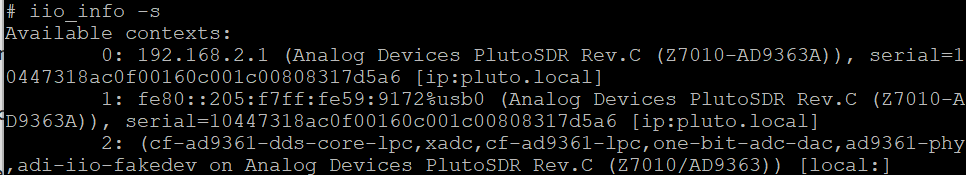
\includegraphics[width=0.9\textwidth]{iio_info_putty.png}}
	\caption{Result of \texttt{iio\_info -s} Command when Executed in Putty}
	\label{fig::iio_info_putty}
\end{figure}

We compare the outputs displayed in the SSH terminal to the outputs of the same command executed in command prompt, a local PC terminal. The output of the updated commanded is shown in Figure \ref{fig::iio_info_cmd}.

\begin{figure}[H]
	\centerline{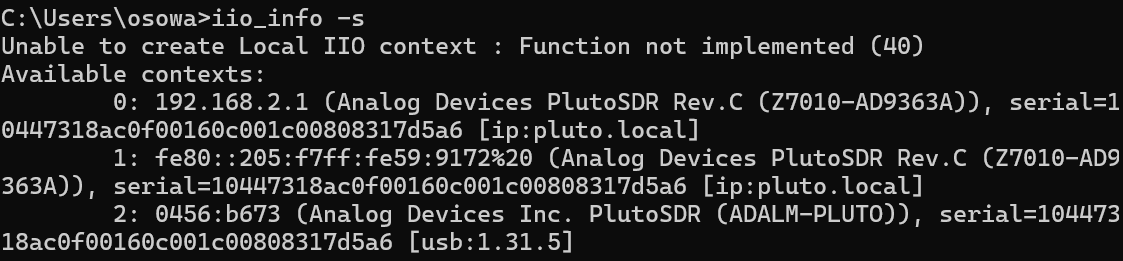
\includegraphics[width=0.9\textwidth]{iio_info_cmd.png}}
	\caption{Result of \texttt{iio\_info -s} Command when Executed in Command Prompt}
	\label{fig::iio_info_cmd}
\end{figure}

The command prompt output contains very similar URIs to the SSH output shown in Figure \ref{fig::iio_info_putty}. Both sets of outputs contain two \texttt{ip:pluto.local} URIs. The printout for one of these local URIs is exactly the same and is associated with an IP address of 192.169.2.1. The other local URI printout is nearly the same. The biggest difference we observe in the SSH and PC terminal outputs is in the final URI. In the ssh terminal, the URI is a local URI (\texttt{local:}). while the command prompt URI is a USB URI (\texttt{usb:1.31.5}). We note that command prompt output also contains an additional warning message, which says ``Unable to create Local IIO context: Function not implemented (40)." This warning message is described in more detail in \cite{analog_devices_libiio_error}. However, it is an expected warning in Windows operating systems. For comparison, we run the same command on the Virtual Machine. The results of this command are displayed in Figure \ref{fig::iio_info_vm}.

\begin{figure}[H]
	\centerline{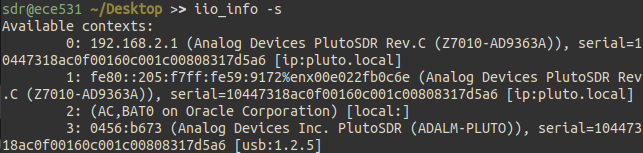
\includegraphics[width=0.9\textwidth]{iio_info_vm.png}}
	\caption{Result of \texttt{iio\_info -s} Command when Executed in Virtual Machine}
	\label{fig::iio_info_vm}
\end{figure}

Compared to the results of Figure \ref{fig::iio_info_cmd}, we see that the IIO context warning message is no longer present. Next, we use the \texttt{iio\_attr -d} command without a device to list all the devices in the PlutoSDR. The output of this command is included in Figure \ref{fig::iio_devices}.

\begin{figure}[H]
	\centerline{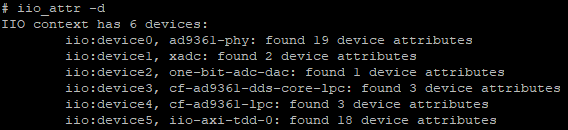
\includegraphics[width=0.75\textwidth]{iio_devices.png}}
	\caption{List of IIO Devices}
	\label{fig::iio_devices}
\end{figure}

Examining the command output, we find that \textit{ad9361-phy} corresponds to \texttt{iio:device0}. Using the following command, we confirm the name of \texttt{iio:device0}.

\begin{center}
\texttt{cat /sys/bus/iio/devices/iio:device0/name}
\end{center}

The outputs of this command are given in Figure \ref{fig::iio_device0_name}.

\begin{figure}[H]
	\centerline{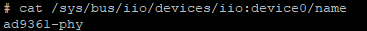
\includegraphics[width=0.5\textwidth]{iio_device0_name.png}}
	\caption{Confirming Name of ``iio:device0"}
	\label{fig::iio_device0_name}
\end{figure}

Examining the command outputs, we find that the name of \texttt{iio:device0} is \textit{ad9361-phy} as expected. We can pass the name of the device as an argument to the \texttt{iio\_attr -d} command to list the attributes of the device. The results of this command are given in Figure \ref{fig::iio_raw_attributes}.

\begin{figure}[H]
	\centerline{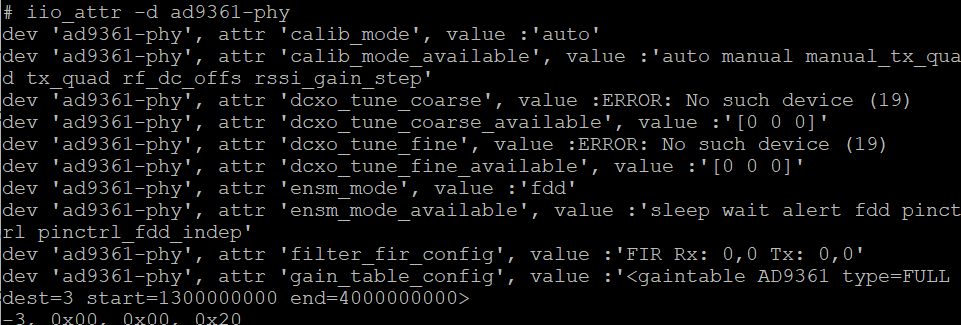
\includegraphics[width=0.9\textwidth]{iio_raw_attributes.png}}
	\caption{Attributes for the \textit{ad9361-phy} Device}
	\label{fig::iio_raw_attributes}
\end{figure}

Note that this command gives the device attributes and their values. However, is is difficult to parse. We can instead display just the attribute names by piping the command output to a combination of \texttt{grep} and \texttt{sed} commands as illustrated in Figure \ref{fig::iio_filtered_attributes}.

\begin{figure}[H]
	\centerline{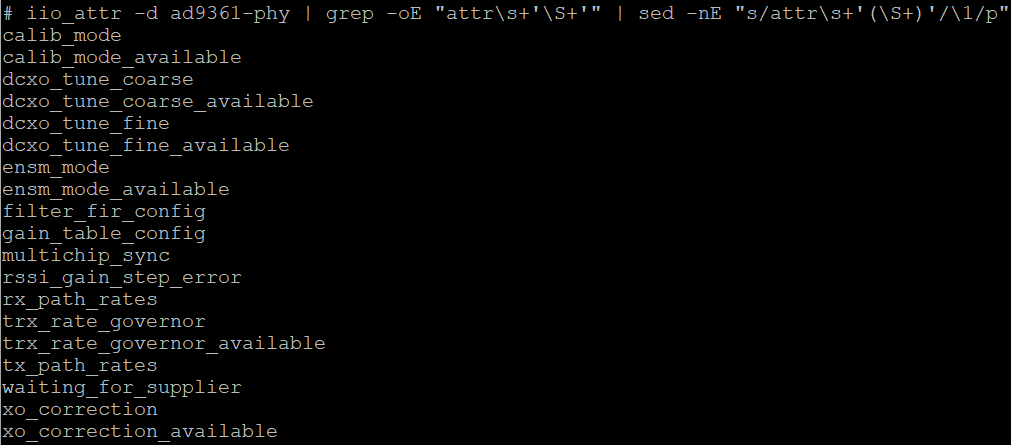
\includegraphics[width=0.9\textwidth]{iio_filtered_attributes.png}}
	\caption{Filtering Output of \texttt{iio\_attr} Command}
	\label{fig::iio_filtered_attributes}
\end{figure}

The \textit{ad9361-phy} device controls the physical (PHY) layer of the transceiver and is responsible for device configuration. In addition to the properties shown above, the \textit{ad9361-phy} device contains multiple channels, which provide access to critical device properties. For example, the \texttt{altvoltage0} and \texttt{altvoltage1} channels provide access to the LO frequencies of the transmitter and receiver, and the \texttt{voltage0} channels provides access to the sample rate, RF bandwidth, and gain control mode. All these parameters will be explored later in the lab.

% Results and discussion of the laboratory experiment, including captured outputs, observations, and responses to laboratory questions.

\subsection{MATLAB Loopback}
\label{section::matlab_loopback_results}

In this section, we perform a loopback test with MATLAB. To prevent discontinuities in the transmitted data, we modify the buffer size in the \texttt{loopback.m} script, so that it contains an integer number of sinusoid periods. To do this, we choose integers $N$ and $M$ to satisfy the following relationship:

\begin{equation}
	\frac{f_o}{f_s} = \frac{M}{N}
\end{equation} 

In the script, $f_o = 300\ \text{Hz}$ and $f_s = 1\ \text{MHz}$. Reducing, we find that $M = 3k$ and $N = 10000k$ where $k$ is any positive integer. We choose $k=3$ to get a buffer size $N = 30000$. We, then, perform a baseline data collect with \textit{Manual} AGC and 24 dB of receive gain. The resulting data is shown in Figure \ref{fig::matlab_loopback_baseline}.

\begin{figure}[H]
	\centerline{\fbox{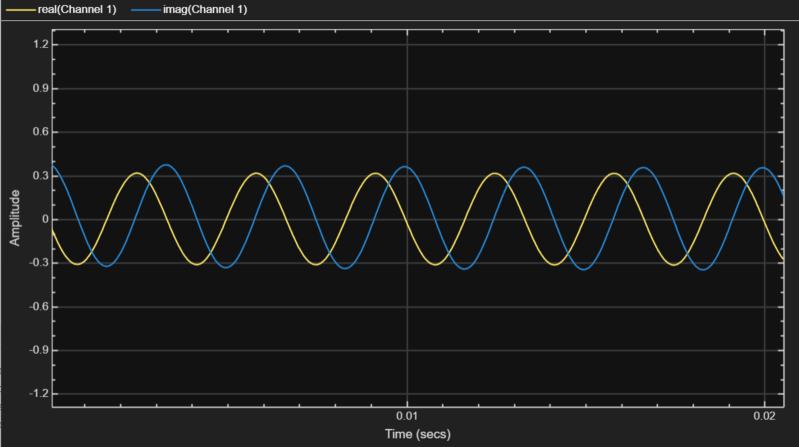
\includegraphics[width=0.8\textwidth]{matlab_loopback_baseline.png}}}
	\caption{Loopback Collect with 24 dB of Receive Gain}
	\label{fig::matlab_loopback_baseline}
\end{figure}

We compare the data collected with \textit{Manual} AGC to data collected using the \textit{AGC Slow Attack} and \textit{AGC Fast Attack} settings. The data collected with the updated AGC settings is shown in Figures \ref{fig::matlab_loopback_agc_slow_attack} and \ref{fig::matlab_loopback_agc_fast_attack}.

\begin{figure}[H]
	\centerline{\fbox{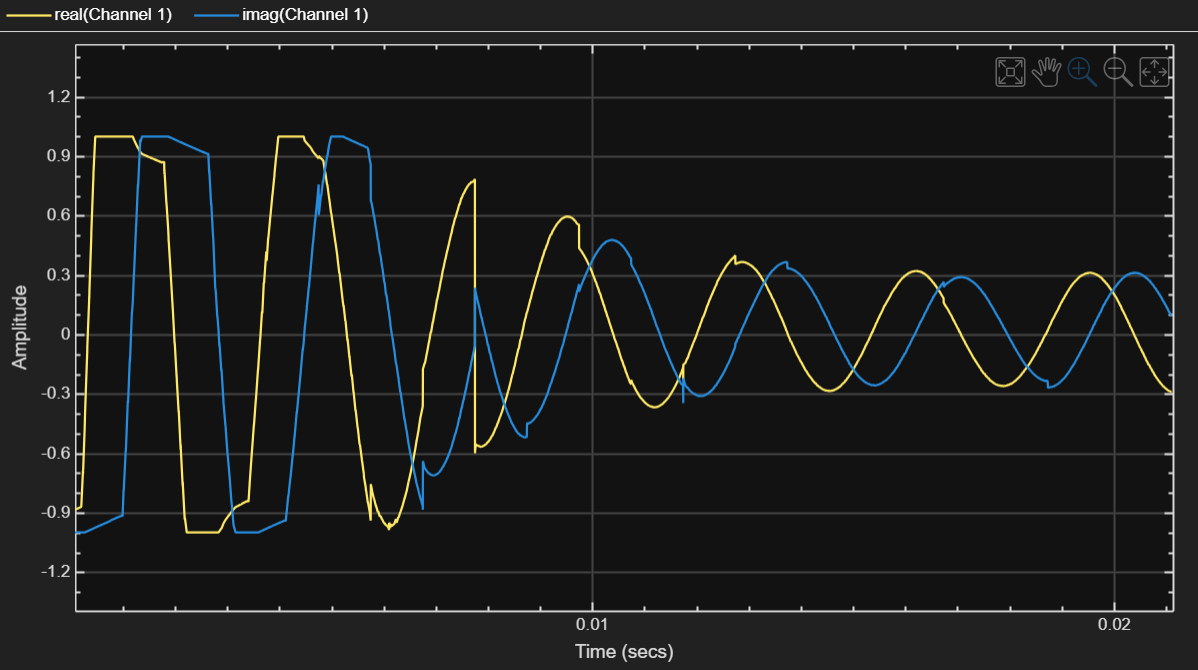
\includegraphics[width=0.8\textwidth]{matlab_loopback_agc_slow_attack.png}}}
	\caption{Loopback Collect using \textit{AGC Slow Attack}}
	\label{fig::matlab_loopback_agc_slow_attack}
\end{figure}

\begin{figure}[H]
	\centerline{\fbox{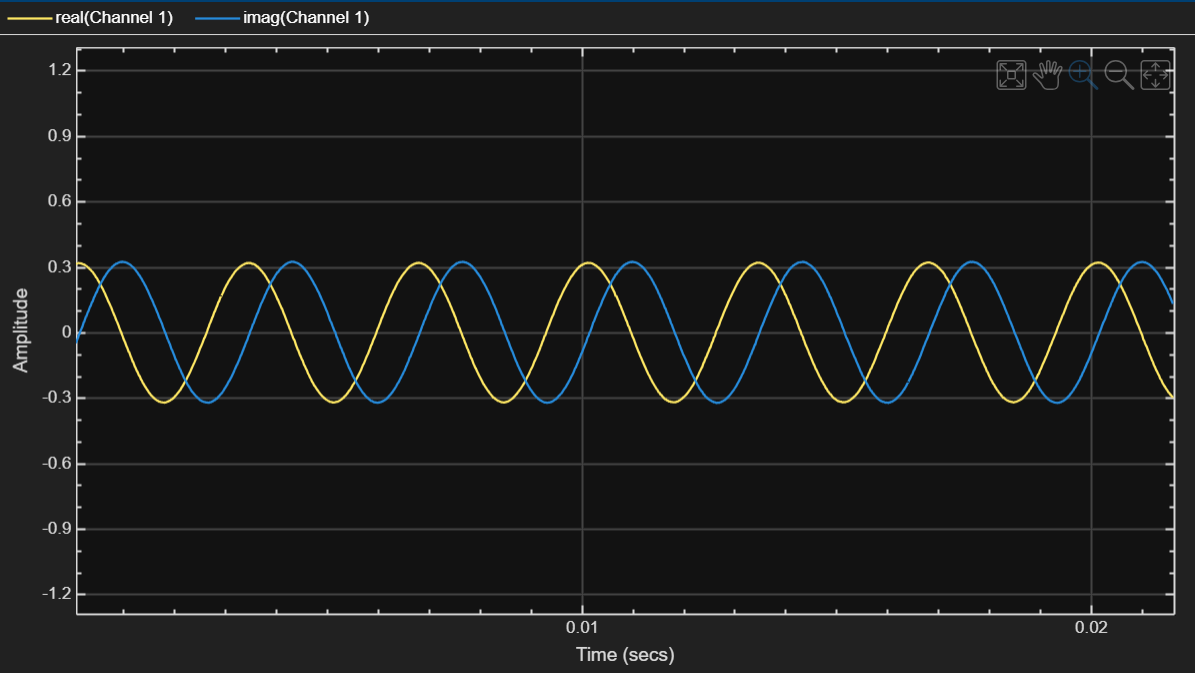
\includegraphics[width=0.8\textwidth]{matlab_loopback_agc_fast_attack.png}}}
	\caption{Loopback Collect using \textit{AGC Fast Attack}}
	\label{fig::matlab_loopback_agc_fast_attack}
\end{figure}

Looking at the data collected with the \textit{Slow AGC Attack} setting, we observe that the first few sinusoid periods are saturated. However, with the \textit{AGC Fast Attack} setting, we don't observe any saturation. This is because the \textit{Slow AGC Attack} algorithm takes more time to reach steady state compared to the \textit{Fast AGC Attack} algorithm.

By adding zeros to the data, we can observe the step response of each AGC algorithm. For these collects, we configure the data to have a duty cycle of 75\% (i.e. the first 75\% of the data is untouched, while the last 25\% is replaced with zeros). The resulting data collected with the \textit{Manual} AGC setting is shown in Figure \ref{fig::matlab_loopback_agc_manual_75p_duty_cycle}.

\begin{figure}[H]
	\centerline{\fbox{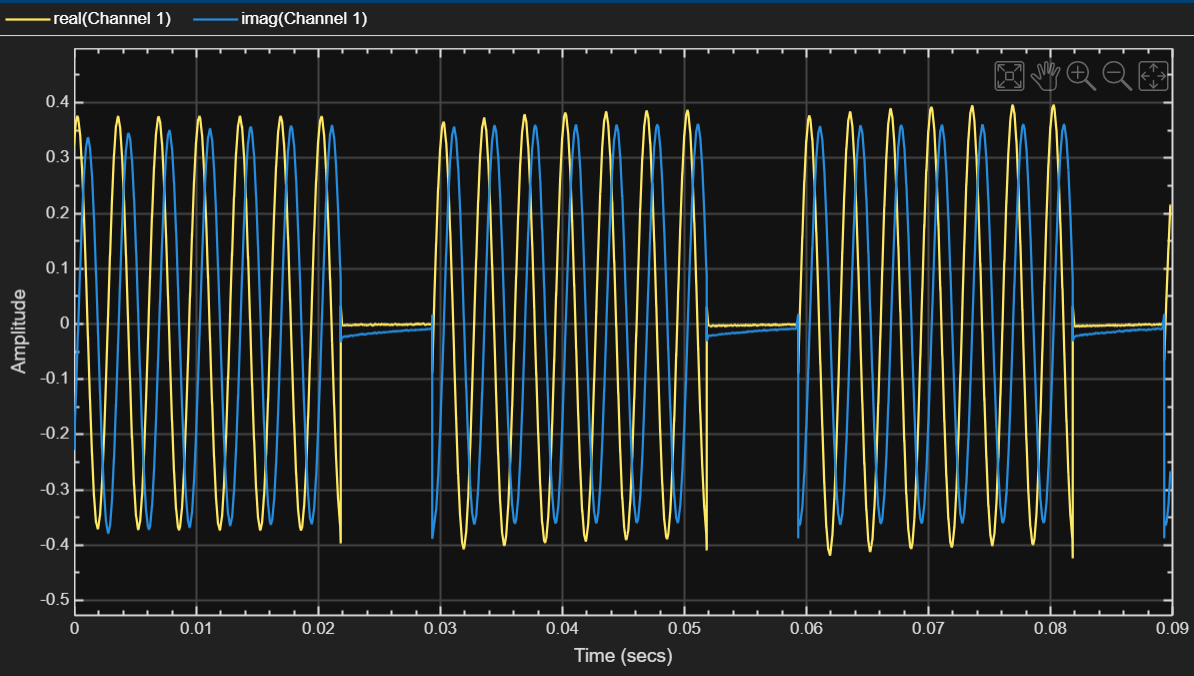
\includegraphics[width=0.8\textwidth]{matlab_loopback_agc_manual_75p_duty_cycle.png}}}
	\caption{75\% Duty Cycle Loopback Collect with \textit{Manual} AGC Setting}
	\label{fig::matlab_loopback_agc_manual_75p_duty_cycle}
\end{figure}

We perform similar collects with the \textit{AGC Slow Attack} and \textit{AGC Fast Attack} settings. The results with the updated AGC settings is shown in Figures \ref{fig::matlab_loopback_agc_slow_attack_75p_duty_cycle} and \ref{fig::matlab_loopback_agc_fast_attack_75p_duty_cycle}.

\begin{figure}[H]
	\centerline{\fbox{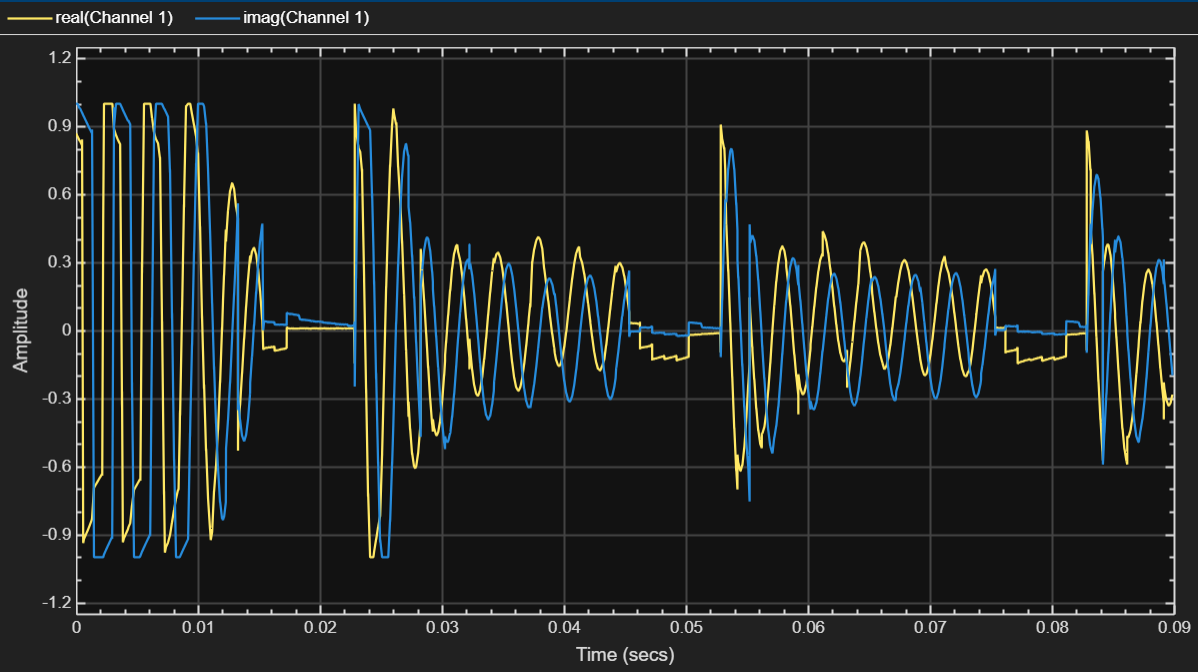
\includegraphics[width=0.8\textwidth]{matlab_loopback_agc_slow_attack_75p_duty_cycle.png}}}
	\caption{75\% Duty Cycle Loopback Collected with \textit{AGC Slow Attack} Setting}
	\label{fig::matlab_loopback_agc_slow_attack_75p_duty_cycle}
\end{figure}

\begin{figure}[H]
	\centerline{\fbox{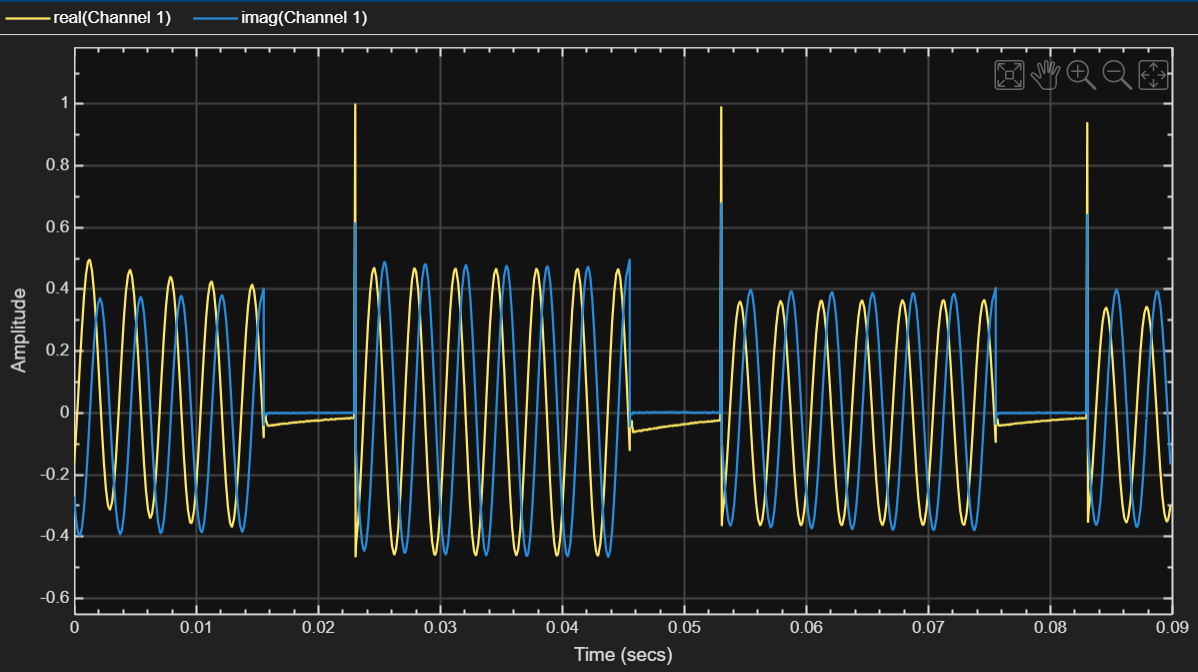
\includegraphics[width=0.8\textwidth]{matlab_loopback_agc_fast_attack_75p_duty_cycle.png}}}
	\caption{75\% Duty Cycle Loopback Collected with \textit{AGC Fast Attack} Setting}
	\label{fig::matlab_loopback_agc_fast_attack_75p_duty_cycle}
\end{figure}

Observing the collected data, we see that the \textit{AGC Fast Attack} Setting quickly converges to the correct headroom, while the 
\textit{AGC Slow Attack} setting takes longer to converge.

Next, we measure the \textit{Gain} setting which results in signal clipping. We find that the signal begins to clip at 34 dB of receive gain. We show the resulting data in Figure \ref{fig::matlab_loopback_agc_manual_34db_gain}. As we increase the gain more, the effects of clipping become more severe resulting in a square wave. We illustrate this in Figure \ref{fig::matlab_loopback_agc_manual_45db_gain}, which shows the results with 45 dB of receive gain.

\begin{figure}[H]
	\centerline{\fbox{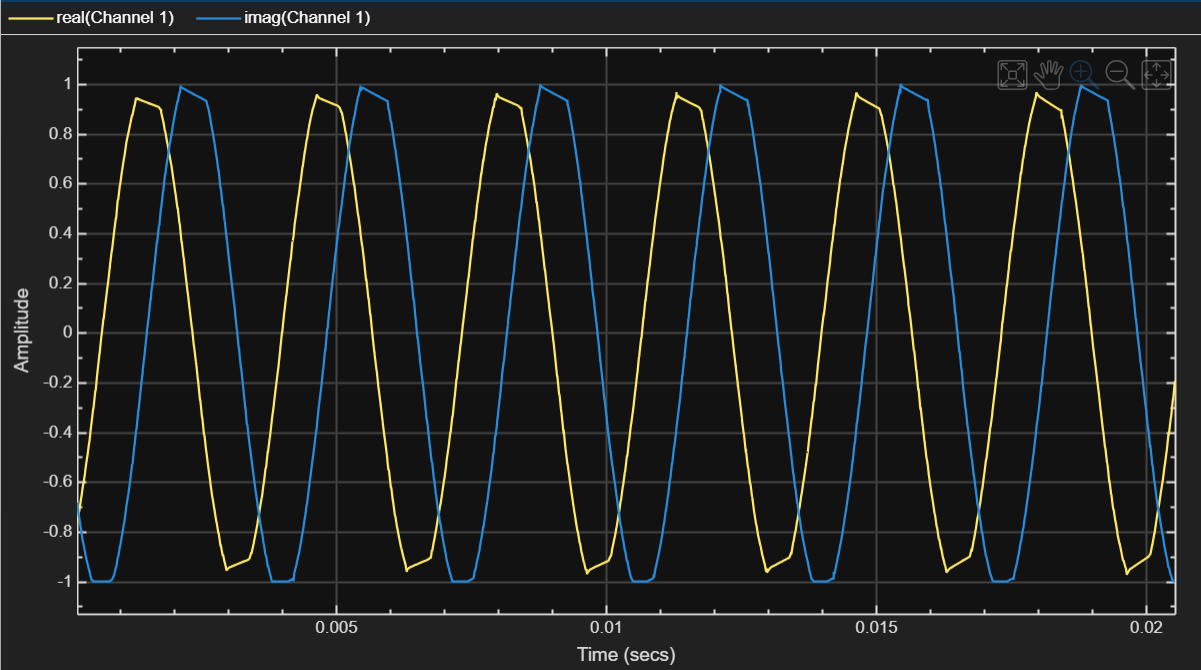
\includegraphics[width=0.8\textwidth]{matlab_loopback_agc_manual_34db_gain.png}}}
	\caption{Data Collected with 34 dB of Receive Gain Resulting in Clipping}
	\label{fig::matlab_loopback_agc_manual_34db_gain}
\end{figure}

\begin{figure}[H]
	\centerline{\fbox{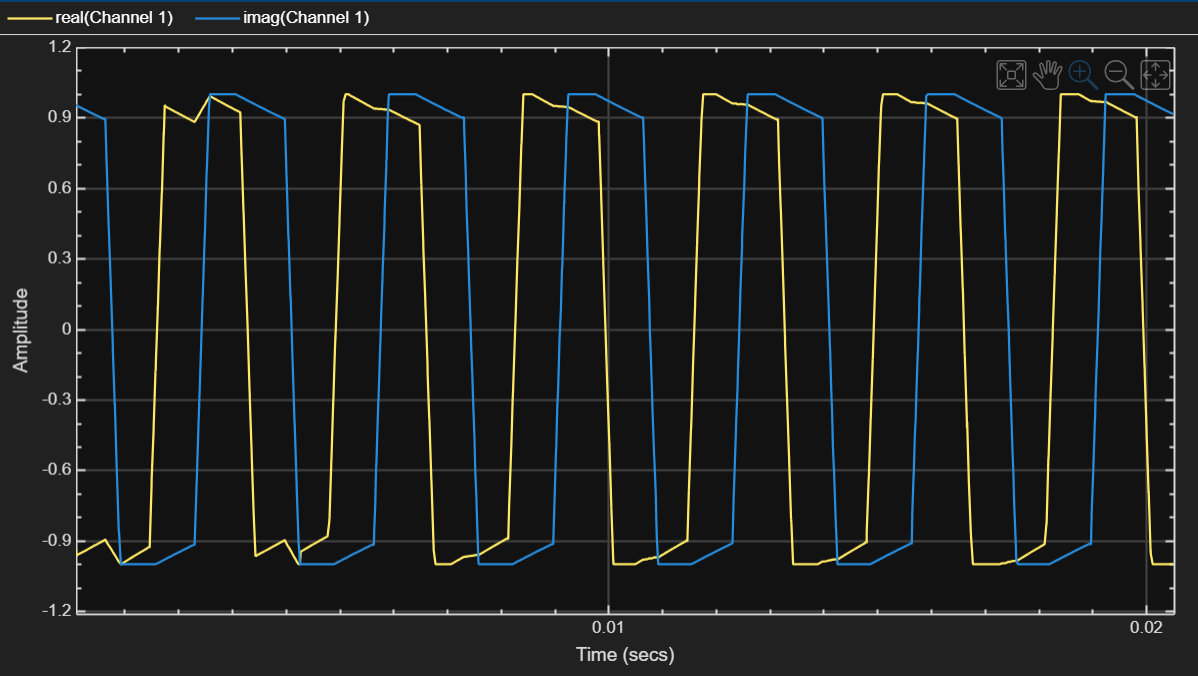
\includegraphics[width=0.8\textwidth]{matlab_loopback_agc_manual_45db_gain.png}}}
	\caption{Data Collected with 45 dB of Receive Gain Resulting in Severe Clipping}
	\label{fig::matlab_loopback_agc_manual_45db_gain}
\end{figure}

\subsection{GNU Radio Loopback}

In this section, we use GNU Radio instead of MATLAB to perform a loopback test. For our experiment, we leverage the GNU Radio flowchart shown in Figure \ref{fig::gnu_radio_loopback_flowchart}. We start the experiment by reviewing the properties of the PlutoSDR blocks (both transmit and receive). Relevant properties for each block are displayed in Figures \ref{fig::general_attributes_pluto_sdr_sink} - \ref{fig::filter_attributes_pluto_sdr_source}.

\begin{figure}[H]
	\centerline{\fbox{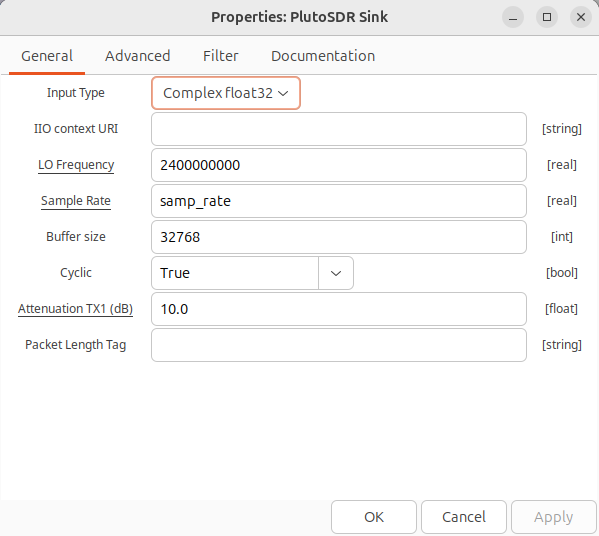
\includegraphics[width=0.5\textwidth]{general_attributes_pluto_sdr_sink.png}}}
	\caption{General Attributes of Pluto SDR Sink}
	\label{fig::general_attributes_pluto_sdr_sink}
\end{figure}

\begin{figure}[H]
	\centerline{\fbox{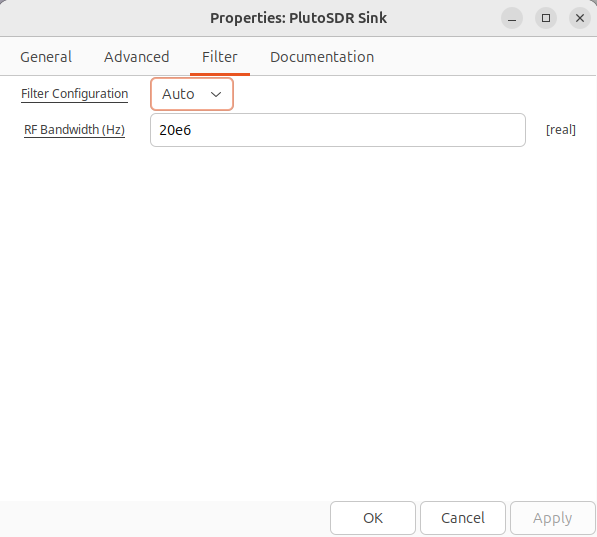
\includegraphics[width=0.5\textwidth]{filter_attributes_pluto_sdr_sink.png}}}
	\caption{Filter Attributes of Pluto SDR Sink}
	\label{fig::filter_attributes_pluto_sdr_sink}
\end{figure}

\begin{figure}[H]
	\centerline{\fbox{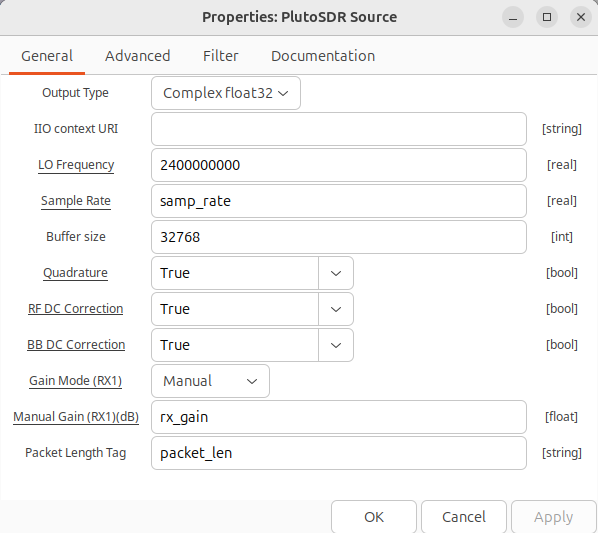
\includegraphics[width=0.5\textwidth]{general_attributes_pluto_sdr_source.png}}}
	\caption{General Attributes of Pluto SDR Source}
	\label{fig::general_attributes_pluto_sdr_source}
\end{figure}

\begin{figure}[H]
	\centerline{\fbox{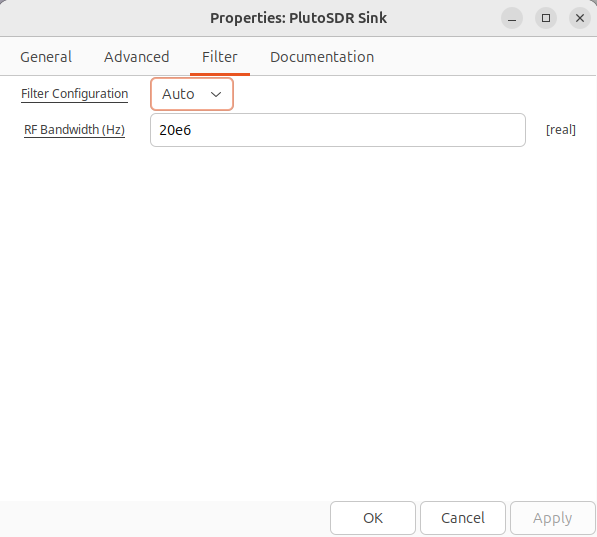
\includegraphics[width=0.5\textwidth]{filter_attributes_pluto_sdr_sink.png}}}
	\caption{Filter Attributes of Pluto SDR Source}
	\label{fig::filter_attributes_pluto_sdr_source}
\end{figure}

In the above figures, the RF bandwidth sets the bandwidth of the analog filters in the transmit and receive paths. The transmit filter removes sampling artifacts and acts as a low-pass filter prior to upconversion. When we mix the signal, we are centering a copy of the spectrum at $+f_c$ and copy at $-f_c$. If our signal is not properly bandlimited, the spectral copies may add together resulting in distortion. The receive filter is responsible for getting rid of the unwanted mixer products and removing out-of-band noise prior to sampling. If our filter bandwidth is too large, this unwanted noise will alias into our spectrum, degrading the SNR. 

Next, we review the cyclic option in the PlutoSDR sink. When the cyclic option is selected, as illustrated in Figure \ref{fig::general_attributes_pluto_sdr_sink}, the PlutoSDR will repeat the first buffer of samples that it receives until the program is stopped. Conversely, when this option is not selected, the PlutoSDR will transmit buffers of samples as it receives them, creating a potentially discontinuous stream of samples which is more difficult to analyze. Additionally, not re-transmitting the same buffer of samples enables us to dedicate more of the USB bandwidth for received data. As long as our buffer size is a multiple of the period, the cyclic option results in the same transmission as a signal source feeding a PlutoSDR Sink with infinite USB bandwidth.

The manual gain control in the PlutoSDR source block disables AGC and allows us to manually set the attenuation. Alternative gain control strategies include slow attack, hybrid, and fast attack. The hybrid gain control option is unique to the GNU Radio block and is not present in the MATLAB API. From an algorithms prespective, the hybrid mode is the same as the slow attack AGC mode with the exception of the gain update counter, which is not present in hybrid mode. This allows the hybrid algorithm to perform more frequent attenuation adjustments.

Using the default receive gain setting of 20 dB, we observe the time and frequency data shown in Figure \ref{fig::gnu_radio_loopback_baseline}.

\begin{figure}[H]
	\centerline{\fbox{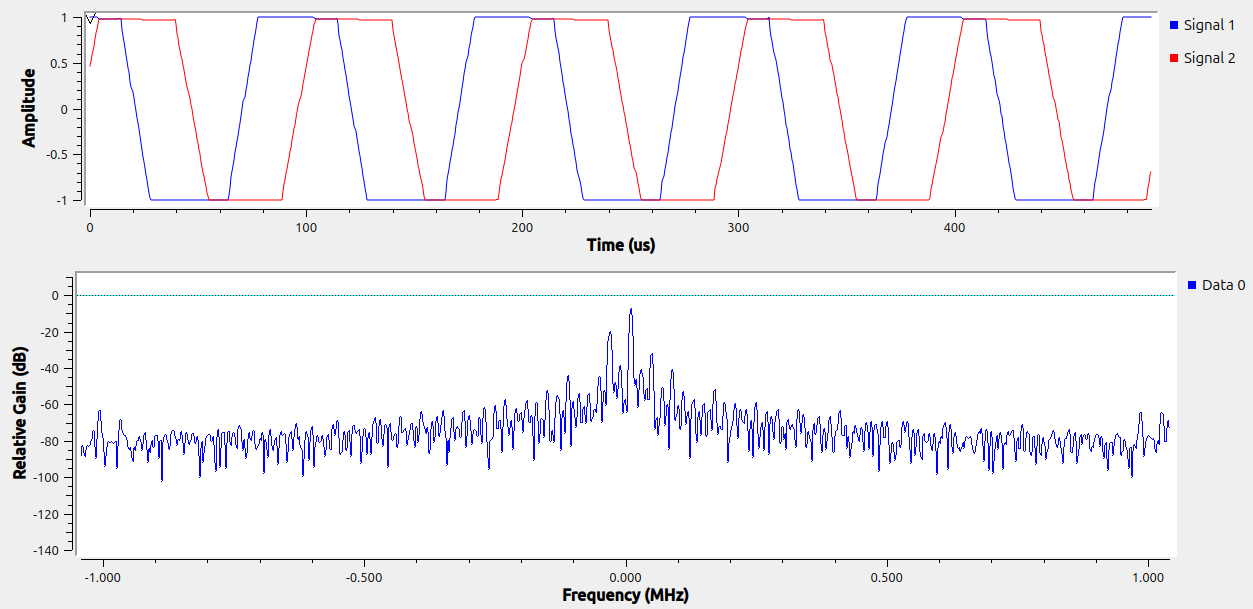
\includegraphics[width=0.8\textwidth]{gnu_radio_loopback_baseline.png}}}
	\caption{GNU Radio Loopback Test with 20 dB of Receive Gain}
	\label{fig::gnu_radio_loopback_baseline}
\end{figure}

With the default settings, the signal has already clipped. From here, we reduce the receive signal gain until we no longer see distortion, which occurs at approximately 12 dB. Figure \ref{fig::gnu_radio_loopback_rx_gain_12dB} shows the collected data with this receive gain setting.

\begin{figure}[H]
	\centerline{\fbox{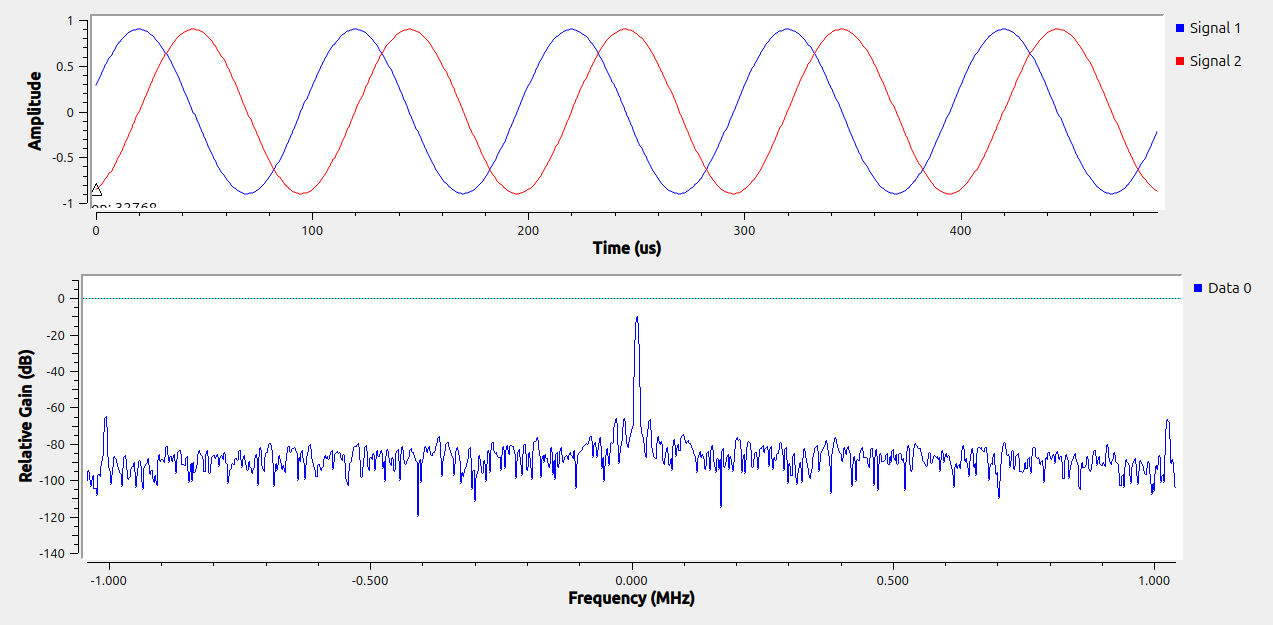
\includegraphics[width=0.8\textwidth]{gnu_radio_loopback_rx_gain_12dB.png}}}
	\caption{GNU Radio Loopback Collect with 12 dB of Receive Gain}
	\label{fig::gnu_radio_loopback_rx_gain_12dB}
\end{figure}

We note that the signal is no longer distorted but is very close to full scale ($\pm 1$). If we increase the receive signal gain to 13 dB, we start to see clipping again as illustrated in Figure \ref{fig::gnu_radio_loopback_rx_gain_13dB}.

\begin{figure}[H]
	\centerline{\fbox{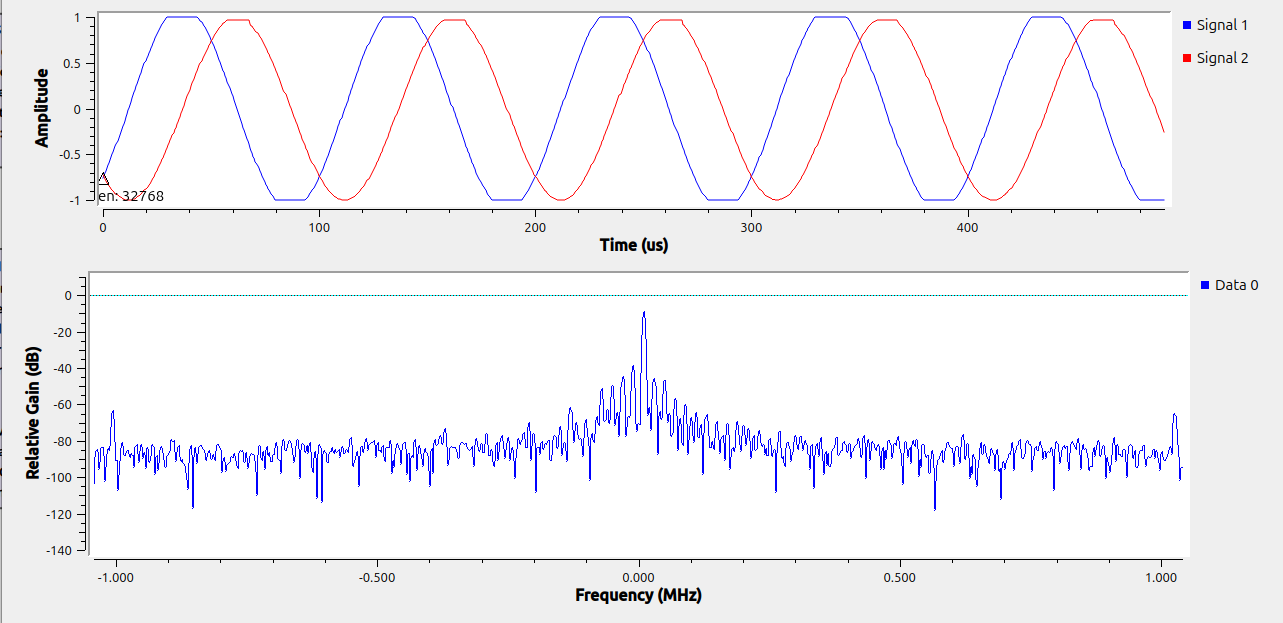
\includegraphics[width=0.8\textwidth]{gnu_radio_loopback_rx_gain_13dB.png}}}
	\caption{GNU Radio Loopback Collect with 13 dB of Receive Gain}
	\label{fig::gnu_radio_loopback_rx_gain_13dB}
\end{figure}

Next, we replace the QT Time Sin" and QT Frequency Sink with the QT GUI Sink and observe the output. The resulting flowchart is shown in Figure \ref{fig::gnu_radio_loopback_flowchart_qt_gui_sink}.

\begin{figure}[H]
	\centerline{\fbox{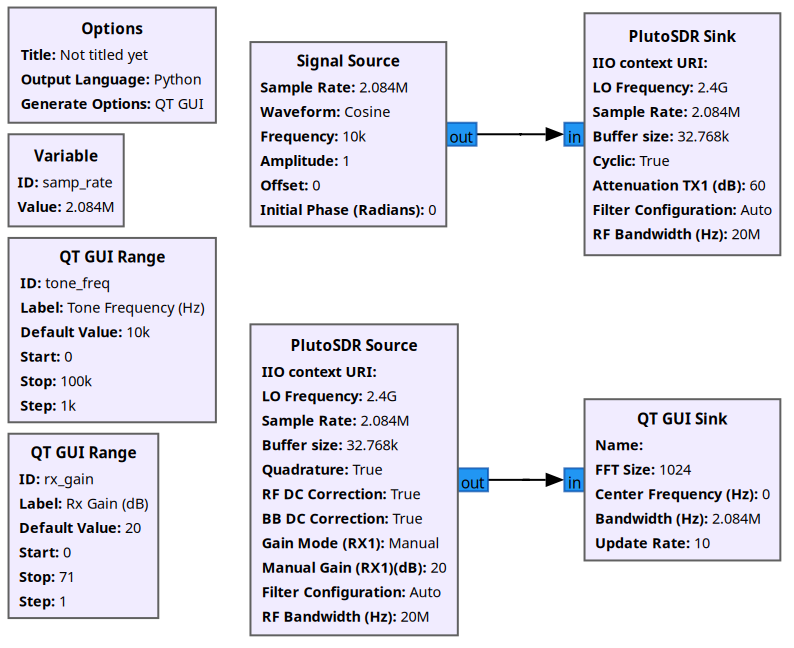
\includegraphics[width=0.5\textwidth]{gnu_radio_loopback_flowchart_qt_gui_sink.png}}}
	\caption{GNU Radio Loopback Flowchart with QT QUI Sink}
	\label{fig::gnu_radio_loopback_flowchart_qt_gui_sink}
\end{figure}

Using the flowchart with 0 dB of receive attenuation, we collect the frequency response shown in Figure \ref{fig::gnu_radio_loopback_qt_gui_sink}.
 
\begin{figure}[H]
	\centerline{\fbox{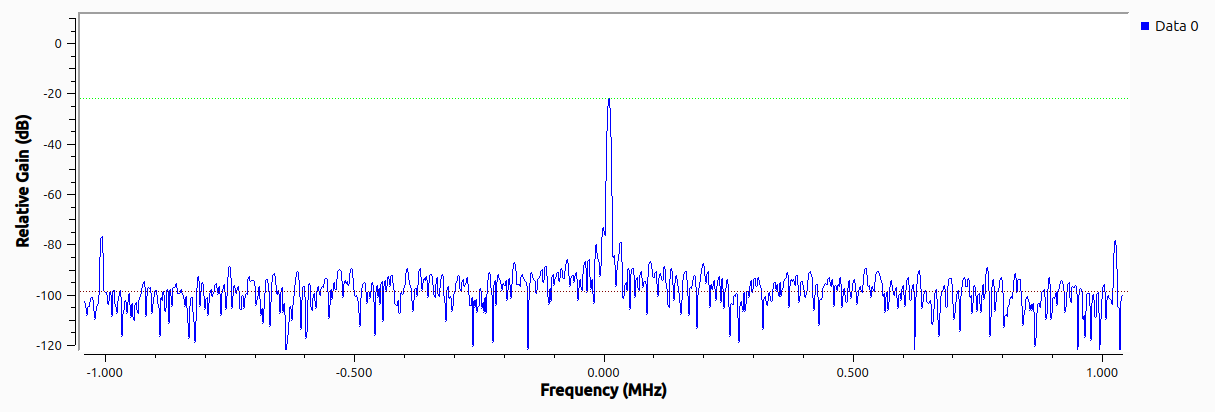
\includegraphics[width=0.8\textwidth]{gnu_radio_loopback_qt_gui_sink.png}}}
	\caption{Frequency Response with QT GUI Sink and 0 dB of Receive Gain}
	\label{fig::gnu_radio_loopback_qt_gui_sink}
\end{figure}

Looking at the frequency response, we see roughly 75 dB of SNR (peak to noise floor). Figure \ref{fig::gnu_radio_loopback_qt_gui_sink_avg_256} shows the frequency response for the same configuration, when we average in power over 256 frames.

\begin{figure}[H]
	\centerline{\fbox{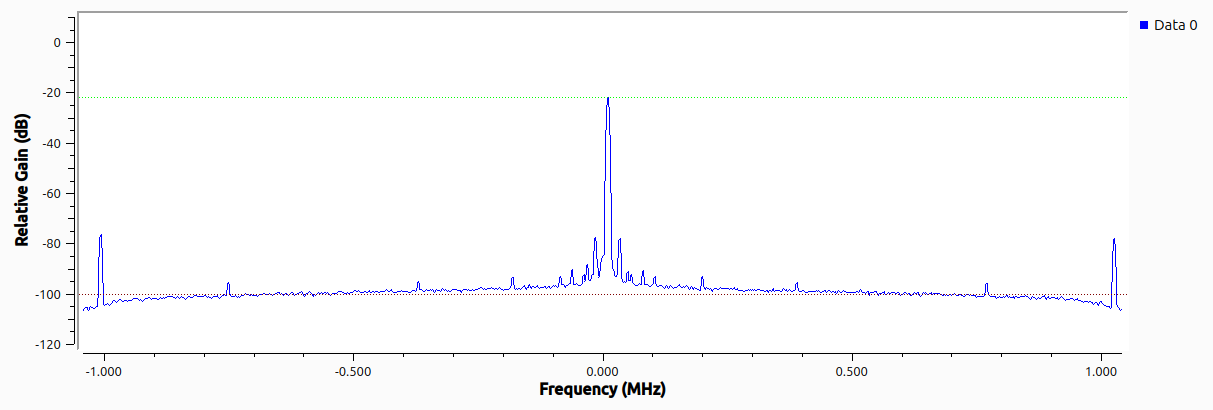
\includegraphics[width=0.8\textwidth]{gnu_radio_loopback_qt_gui_sink_avg_256.png}}}
	\caption{Frequency Response Averaged Over 256 Frames}
	\label{fig::gnu_radio_loopback_qt_gui_sink_avg_256}
\end{figure}

Comparing Figures \ref{fig::gnu_radio_loopback_qt_gui_sink} and \ref{fig::gnu_radio_loopback_qt_gui_sink_avg_256}, we see that integrating multiple frames of the FFT output reduces the variance of the noise, allowing us to better visualize the frequency response of the signal. 

Using a different window will change the frequency response sidelobe levels and rolloff. However, when we reduce sidelobe levels we also increase the mainlobe width. Compare Figure \ref{fig::gnu_radio_loopback_qt_gui_sink_avg_256} which uses a Blackman-Harris window to Figure \ref{fig::gnu_radio_loopback_qt_gui_sink_rect_win} which uses a rectangular window. The sidelobes of the frequency response are substantially lower when the Blackman-Harris window is used. However, the frequency response mainlobe is also much wider.

\begin{figure}[H]
	\centerline{\fbox{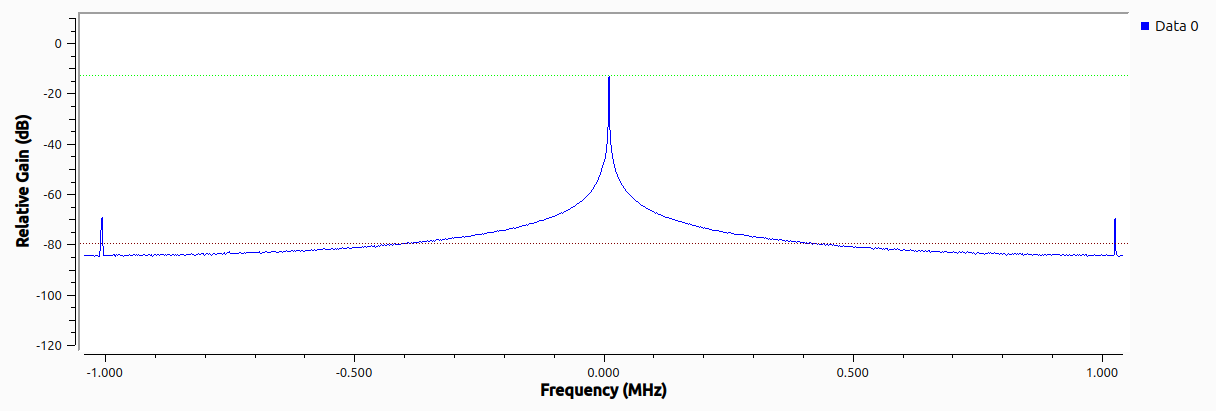
\includegraphics[width=0.8\textwidth]{gnu_radio_loopback_qt_gui_sink_rect_win.png}}}
	\caption{Frequency Response Using Rectangular Window Instead of Blackman-Harris Window}
	\label{fig::gnu_radio_loopback_qt_gui_sink_rect_win}
\end{figure}

The PlutoSDR uses a quadrature mixer to mix the DAC output to the correct frequency. The output of a quadrature mixer is given as follows:
\begin{align}
	y(t) &= \cos(2{\pi}f_ct)\text{Re}\{x(t)\} - \sin(2{\pi}f_ct)\text{Im}\{x(t)\} \\
	&= \text{Re}\{(\text{Re}\{x(t)\} + j\text{Im}\{x(t)\})(\cos(2{\pi}f_ct) + j\sin(2{\pi}f_ct))\} \\
	&= \text{Re}\{X(t)e^{j2{\pi}f_ct}\}
\end{align}

In other words, the transmitted spectrum will be the DAC spectrum centered about $f_c$ and mirrored about the origin. For the PlutoSDR, $f_c$ is the LO frequency. Therefore, our transmitted frequency will be the sinusoid frequency plus the LO frequency. Substituting the parameters from our experiment (10 kHz and 2.4 GHz), we find that our transmitted frequency is 2.40001 GHz. 

\subsection{GNU Radio as a libIIO Client}

In this experiment, we performed a loopback test using the generic IIO blocks shown in Figure \ref{fig::generic_iio_blocks} instead of the PlutoSDR Source and Sink blocks. Most of the PlutoSDR properties displayed in Figures \ref{fig::general_attributes_pluto_sdr_sink} through \ref{fig::filter_attributes_pluto_sdr_source} can now be set with the IIO Attribute Sink. Each IIO Attribute Sink must be fed with a message, which can be created with an IIO Attribute Updater. However, the IIO Attribute Updater has a broken callback function in GNU Radio 3.10.9.2 \cite{analog_devices_broken_iio_block}. As a result, the IIO Attribute Updater cannot be used with a slider. To work around this, I wrote an embedded block which sends a message at the start of the run and every time its input changes. I wrapped this custom block and the IIO Attribute sink into the hierarchy block shown in Figure \ref{fig::iio_input_channel_attribute}.

\begin{figure}[H]
	\centerline{\fbox{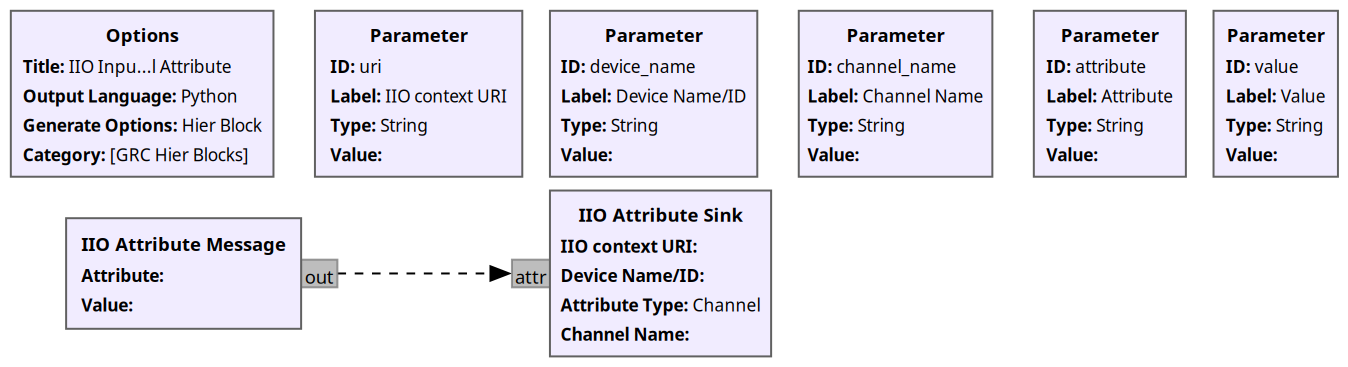
\includegraphics[width=0.8\textwidth]{iio_input_channel_attribute.png}}}
	\caption{Hierarchy Block to Set IIO Channel Attributes}
	\label{fig::iio_input_channel_attribute}
\end{figure}

The PlutoSDR Source and Sink blocks also leverage a programmable FIR. This programmable FIR requires a file to be written to the \texttt{filter\_fir\_config} attribute of the \texttt{ad9361-phy} device with an IIO Attribute Sink. After loading the filter, the \texttt{filter\_fir\_en} attribute needs to be written to the \texttt{voltage0} channel. I created a custom python block to create both of these messages and coordinate their timing. I then wrapped the custom block in another hierarchy block, so I could easily leverage it in the source and sink. The resulting hierarchy block is shown in Figure \ref{fig::iio_fir_config}.

\begin{figure}[H]
	\centerline{\fbox{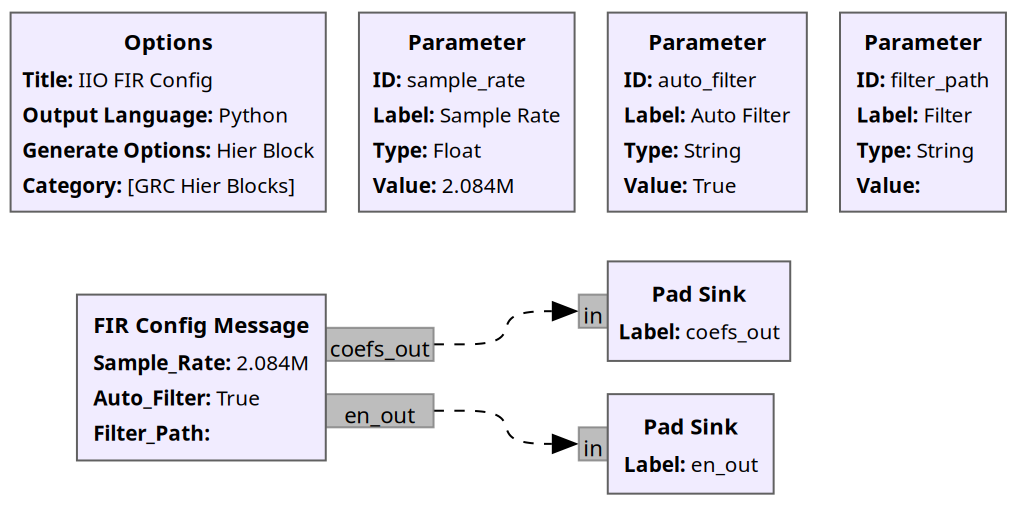
\includegraphics[width=0.5\textwidth]{iio_fir_config.png}}}
	\caption{Hierarchy Block which Create Messages to Configure the Programmable FIR}
	\label{fig::iio_fir_config}
\end{figure}

Using the previously described hierarchy blocks, I created an additional layer of hierarchy blocks to function as the Pluto Source and Sink. These hierarchy blocks are shown in Figure \ref{fig::pluto_iio_device_source} and Figure \ref{fig::pluto_iio_device_sink}.

\begin{figure}[H]
	\centerline{\fbox{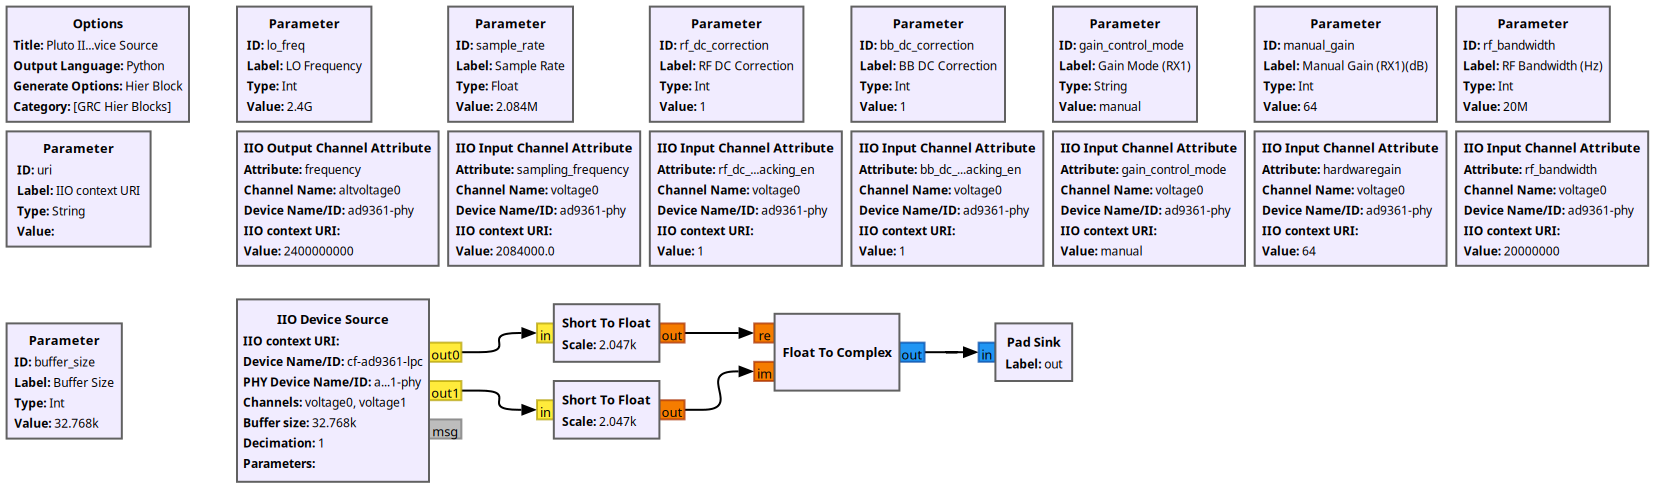
\includegraphics[width=0.9\textwidth]{pluto_iio_device_source.png}}}
	\caption{Hierarchy Block which Functions as Pluto Source}
	\label{fig::pluto_iio_device_source}
\end{figure}

\begin{figure}[H]
	\centerline{\fbox{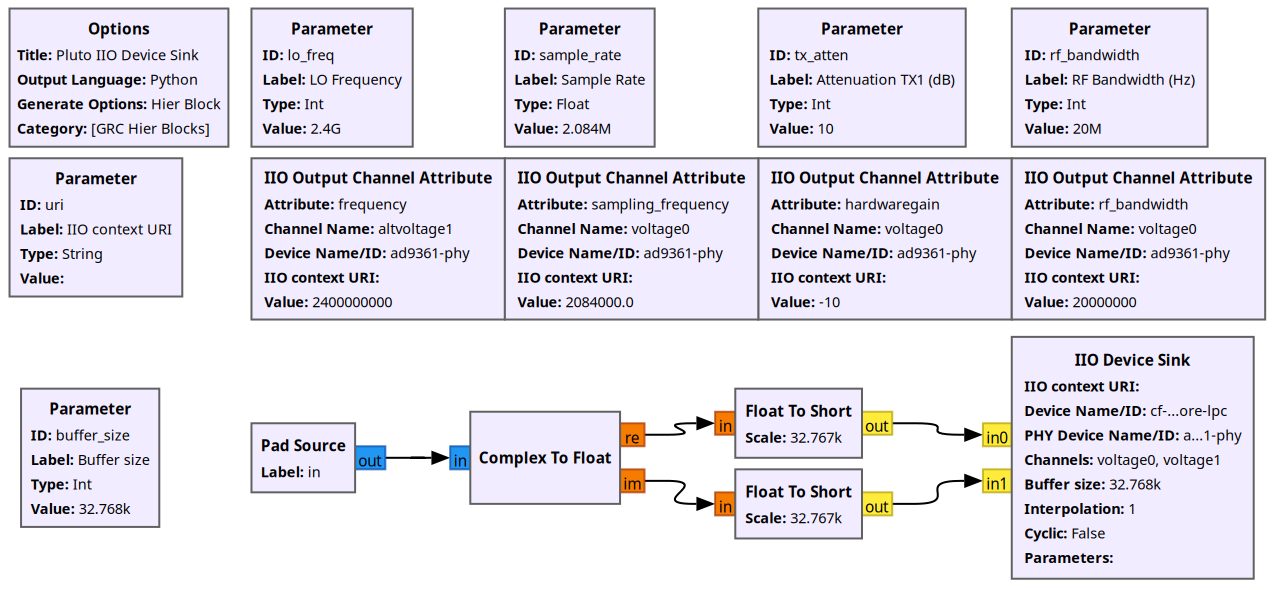
\includegraphics[width=0.9\textwidth]{pluto_iio_device_sink.png}}}
	\caption{Hierarchy Block which Functions as Pluto Sink}
	\label{fig::pluto_iio_device_sink}
\end{figure}

Both the hierarchy blocks shown above use IIO Channel Attribute blocks to set block parameters. Each of the IIO Channel Attribute blocks get the same arguments as the equivalent \texttt{iio\_attr} command. The hierarchy blocks also leverage IIO FIR Configuration blocks to configure the programmable FIR. The source block uses an IIO device source to grab buffers of samples from the ADC. These samples are then scaled and converted to complex floats for processing. In a similar manner, the sink block converts comnplex floats to complex shorts. Then, it uses an IIO device sink to push buffers of samples to the DAC. 

Using the Generic IIO Sink and Source blocks shown above, we create a top-level GNU flowchart for our experiment. This flowchart is shown in Figure \ref{fig::gnu_radio_loopback_generic_iio} and is nearly identical to the flowchart shown in Figure \ref{fig::gnu_radio_loopback_flowchart}.

\begin{figure}[H]
	\centerline{\fbox{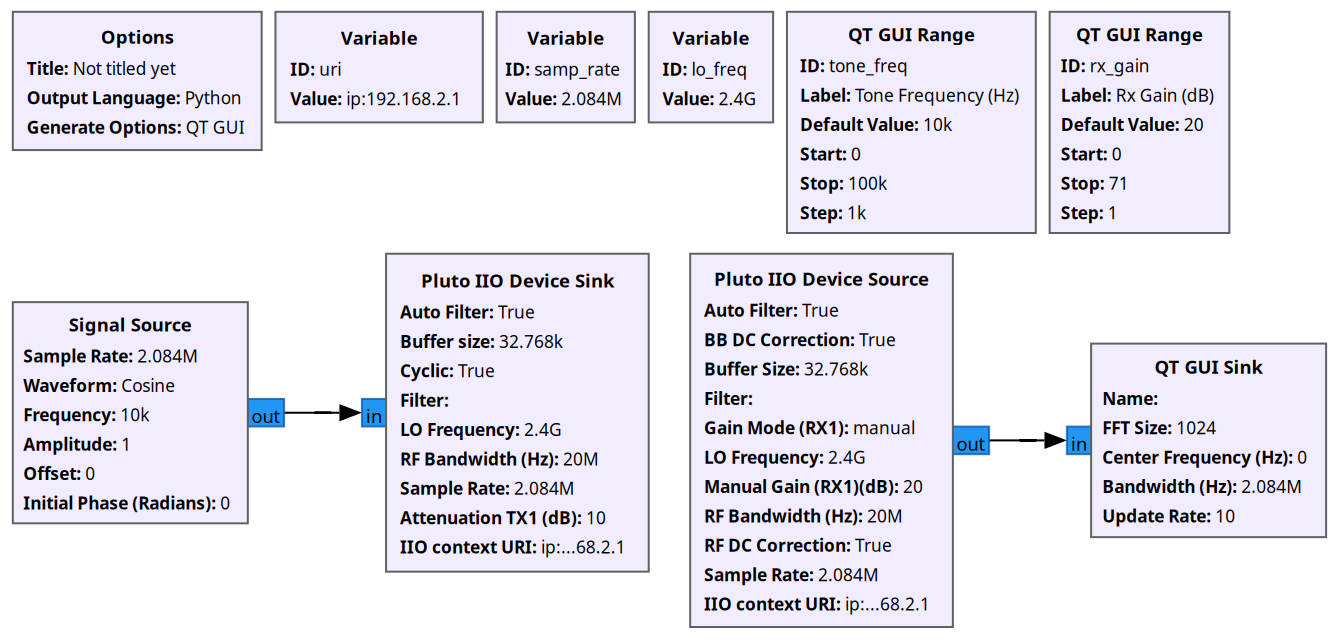
\includegraphics[width=0.6\textwidth]{gnu_radio_loopback_generic_iio.png}}}
	\caption{GNU Flowchart for Loopback Test with Generic IIO Blocks}
	\label{fig::gnu_radio_loopback_generic_iio}
\end{figure}

Using the updated flowchart, we repeat the experiment described in Section \ref{section::gnu_radio_loopback}. Note that our initial flowchart contains the QT GUI Sink instead of the QT GUI Time Sink. This is okay for our experiment because the QT GUI Sink contains all the functionality of the QT GUI Time Sink.

Repeating what was previously done, we measure the receive gain at which clipping occurs. Figure \ref{fig::gnu_radio_loopback_generic_iio_rx_gain_12dB} and Figure 
\ref{fig::gnu_radio_loopback_generic_iio_rx_gain_13dB} show the resulting time-domain data with 12 and 13 dB of receive gain. Looking at the captured data, we conclude that clipping occurs at 13 dB, the same gain we measured earlier.
 
\begin{figure}[H]
	\centerline{\fbox{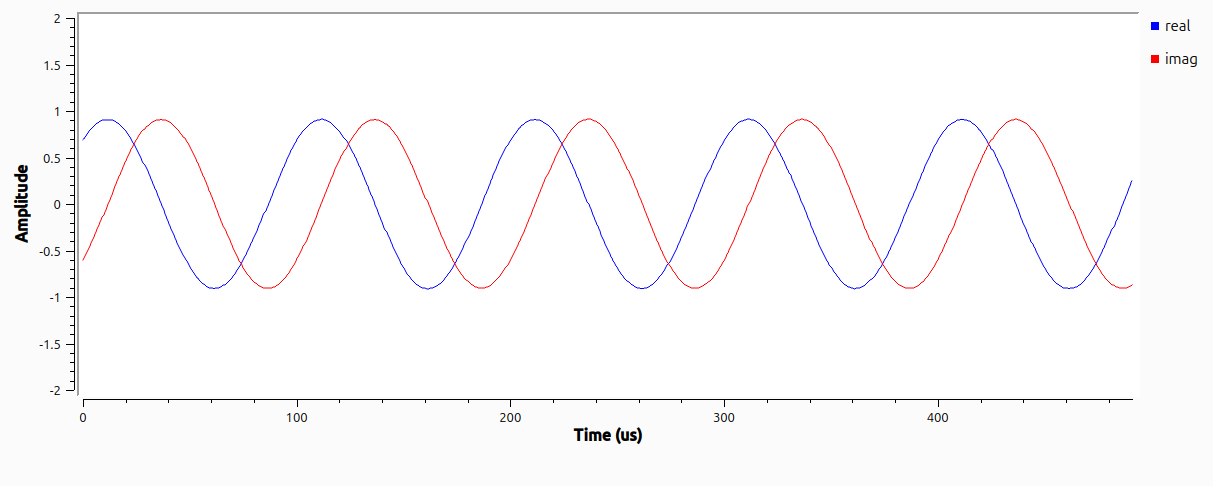
\includegraphics[width=0.8\textwidth]{gnu_radio_loopback_generic_iio_rx_gain_12dB.png}}}
	\caption{Time Domain Loopback Data with 12 dB of Receive Gain}
	\label{fig::gnu_radio_loopback_generic_iio_rx_gain_12dB}
\end{figure}

\begin{figure}[H]
	\centerline{\fbox{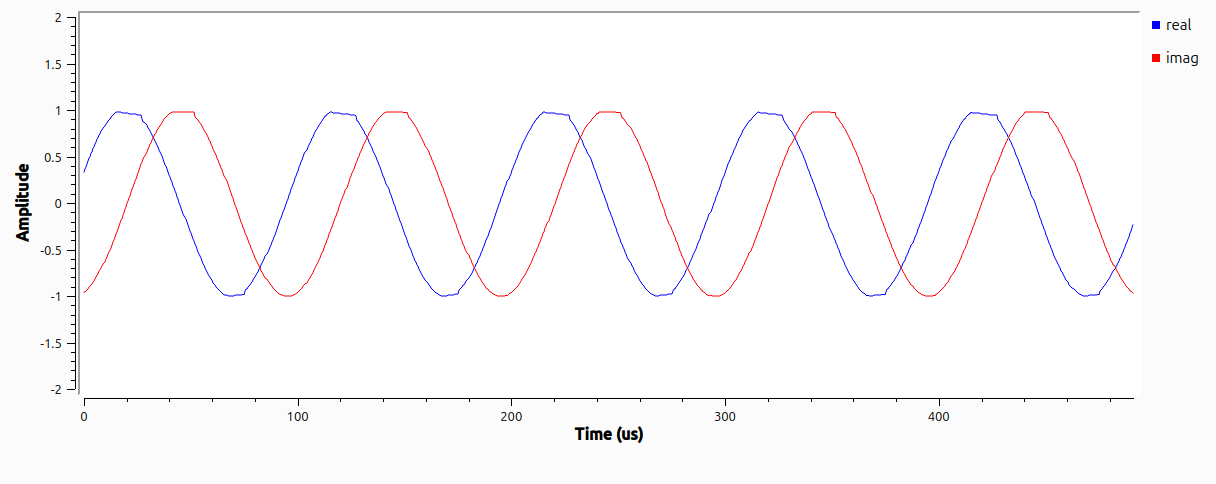
\includegraphics[width=0.8\textwidth]{gnu_radio_loopback_generic_iio_rx_gain_13dB.png}}}
	\caption{Time Domain Loopback Data with 13 dB of Receive Gain}
	\label{fig::gnu_radio_loopback_generic_iio_rx_gain_13dB}
\end{figure}

Next, we capture the frequency response with 0 dB of receive gain and average it across 256 frames. We capture this result in Figure \ref{fig::gnu_radio_loopback_generic_iio_avg_256} and note that it is nearly identical to the data we captured in Figure \ref{fig::gnu_radio_loopback_qt_gui_sink_avg_256}.

\begin{figure}[H]
	\centerline{\fbox{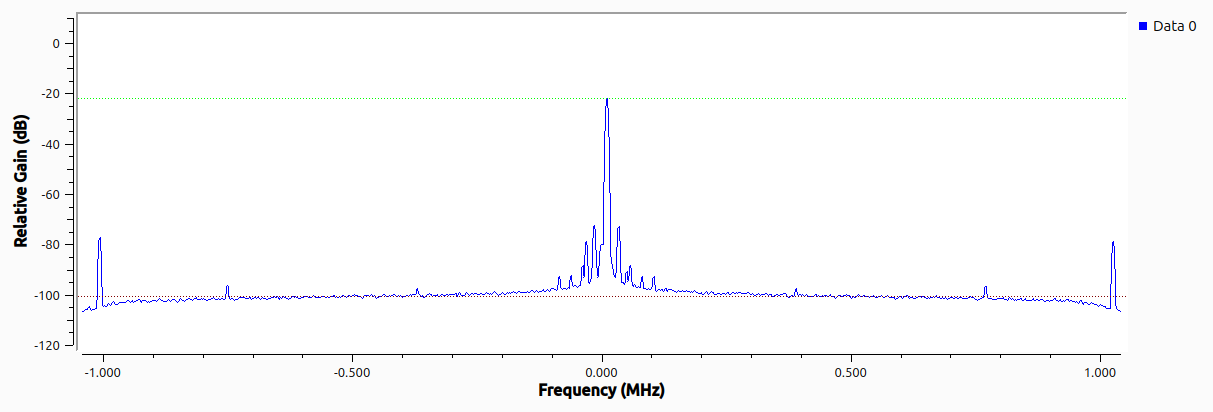
\includegraphics[width=0.8\textwidth]{gnu_radio_loopback_generic_iio_avg_256.png}}}
	\caption{Frequency Response Averaged Over 256 Frames}
	\label{fig::gnu_radio_loopback_generic_iio_avg_256}
\end{figure}

In a similar manner, we recollect the frequency with a rectangular window. These results are shown in Figure \ref{fig::gnu_radio_loopback_generic_iio_rect_win} and are nearly identical to the ones we captured in Figure \ref{fig::gnu_radio_loopback_qt_gui_sink_rect_win}.

\begin{figure}[H]
	\centerline{\fbox{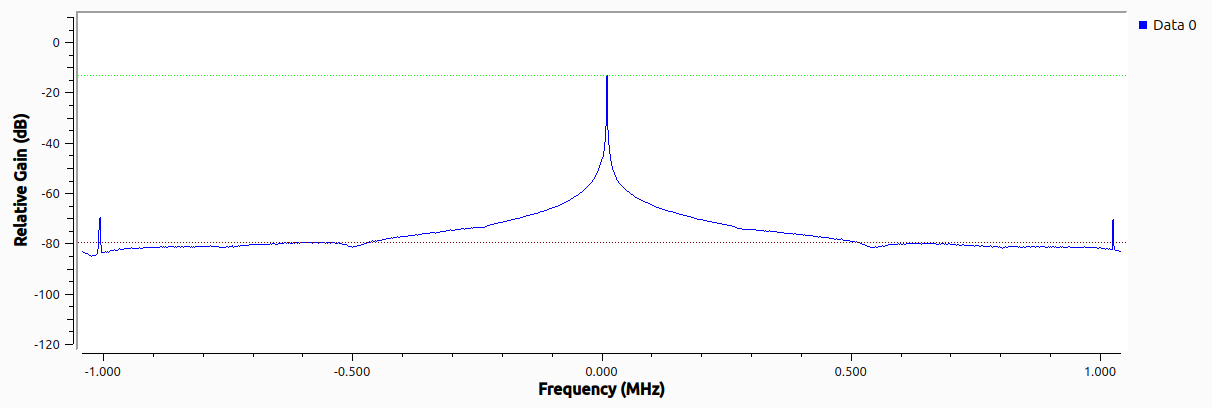
\includegraphics[width=0.8\textwidth]{gnu_radio_loopback_generic_iio_rect_win.png}}}
	\caption{Frequency Response Using Rectangular Window Instead of Blackman-Harris Window}
	\label{fig::gnu_radio_loopback_generic_iio_rect_win}
\end{figure}

Then, we reduce the LO frequency to 915 MHz and observe the frequency response, which is included in Figure \ref{fig::gnu_radio_loopback_generic_iio_915_MHz_lo}.

\begin{figure}[H]
	\centerline{\fbox{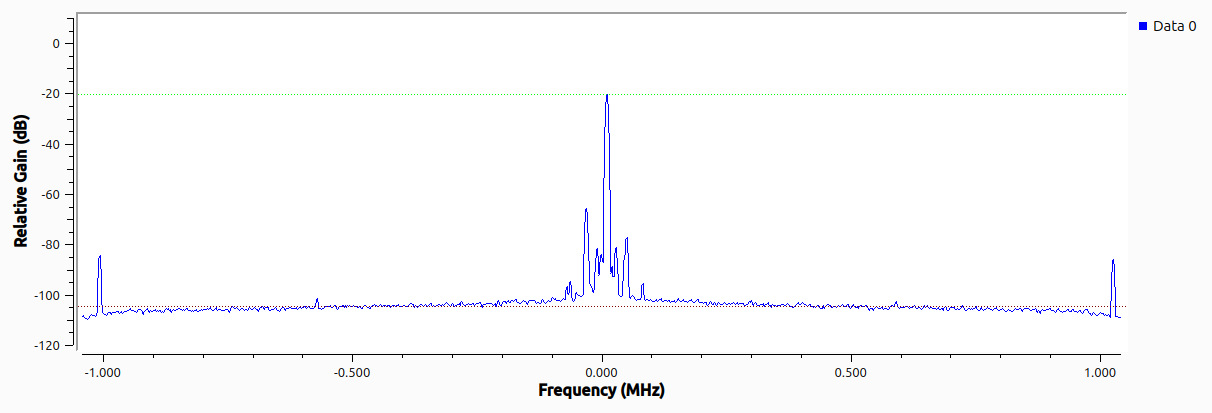
\includegraphics[width=0.8\textwidth]{gnu_radio_loopback_generic_iio_915_MHz_lo.png}}}
	\caption{Frequency Response when LO Frequency is Changed to 915 MHz}
	\label{fig::gnu_radio_loopback_generic_iio_915_MHz_lo}
\end{figure}

Note that the updated frequency response is approximately the same because we are performing baseband sampling. However, we can confirm the LO frequency change with the \texttt{iio\_attr} commands shown in Figure \ref{fig::iio_attr_confirm_lo_frequency}.

\begin{figure}[H]
	\centerline{\fbox{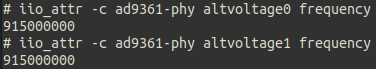
\includegraphics[width=0.5\textwidth]{iio_attr_confirm_lo_frequency.png}}}
	\caption{Confirming a 915MHz LO Frequency with \texttt{iio\_attr} Commands}
	\label{fig::iio_attr_confirm_lo_frequency}
\end{figure}

Note that the \texttt{altvoltage0} channel gives us the \texttt{RX\_LO} frequency, while the \texttt{altvoltage1} channel gives us the \texttt{TX\_LO} frequency. After updating the LO frequency, we also increase the sampling rate to 4 MHz. The updated frequency response is shown in Figure \ref{fig::gnu_radio_loopback_generic_iio_4MSPS} and has a frequency span of $\pm 2 \text{MHz}$.

\begin{figure}[H]
	\centerline{\fbox{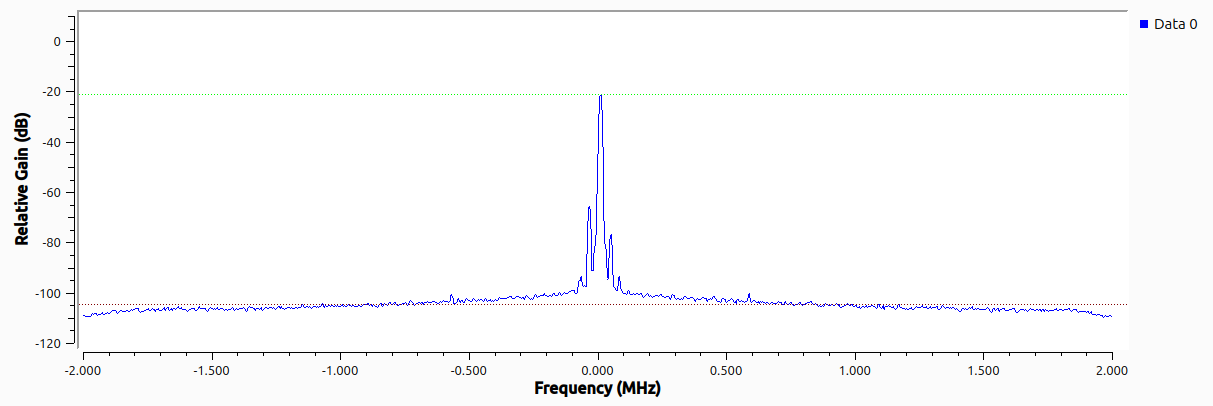
\includegraphics[width=0.8\textwidth]{gnu_radio_loopback_generic_iio_4MSPS.png}}}
	\caption{Frequency Response when the Sampling Rate is Increased to 4 MHz}
	\label{fig::gnu_radio_loopback_generic_iio_4MSPS}
\end{figure}

In a similar manner to what was shown above, we confirm the updated sampling rate using the \texttt{iio\_attr} commands shown in Figure \ref{fig::iio_attr_confirm_sampling_rate}.

\begin{figure}[H]
	\centerline{\fbox{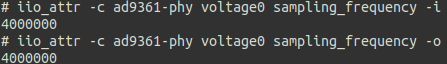
\includegraphics[width=0.5\textwidth]{iio_attr_confirm_sampling_rate.png}}}
	\caption{Confirming a 4MHz Sampling Rate with \texttt{iio\_attr} Commands}
	\label{fig::iio_attr_confirm_sampling_rate}
\end{figure}

\subsection{Measurements and the Radio}

In this section, we use loopback SDR data collected in MATLAB to measure the SNR. To perform this measurement, we follow the procedure outlined in Section \ref{section::snr_measurement}. When the transmitted signal power suddenly drops, the received signal power takes time to converge due to IIR filters in the chain. Measuring the noise power when the received signal power is still decaying can lead to artificially high noise power estimates. To mitigate these effects, we increase the buffer size, which in turn increases the duration of the high and low-energy signal segments. For the collects that follow, we have specifically configured the buffer size to be 100,000 samples.

We start by measuring the SNR when the receive signal gain is 50 dB and the transmit signal gain is -70 dB. The signal power is plotted in Figure \ref{fig::snr_manual_agc_50db_rx_gain_70db_tx_atten}. In the figure, we also mark the regions we used for power measurements. Note that we specifically have avoided the regions with decaying signal power.

\begin{figure}[H]
	\centerline{\fbox{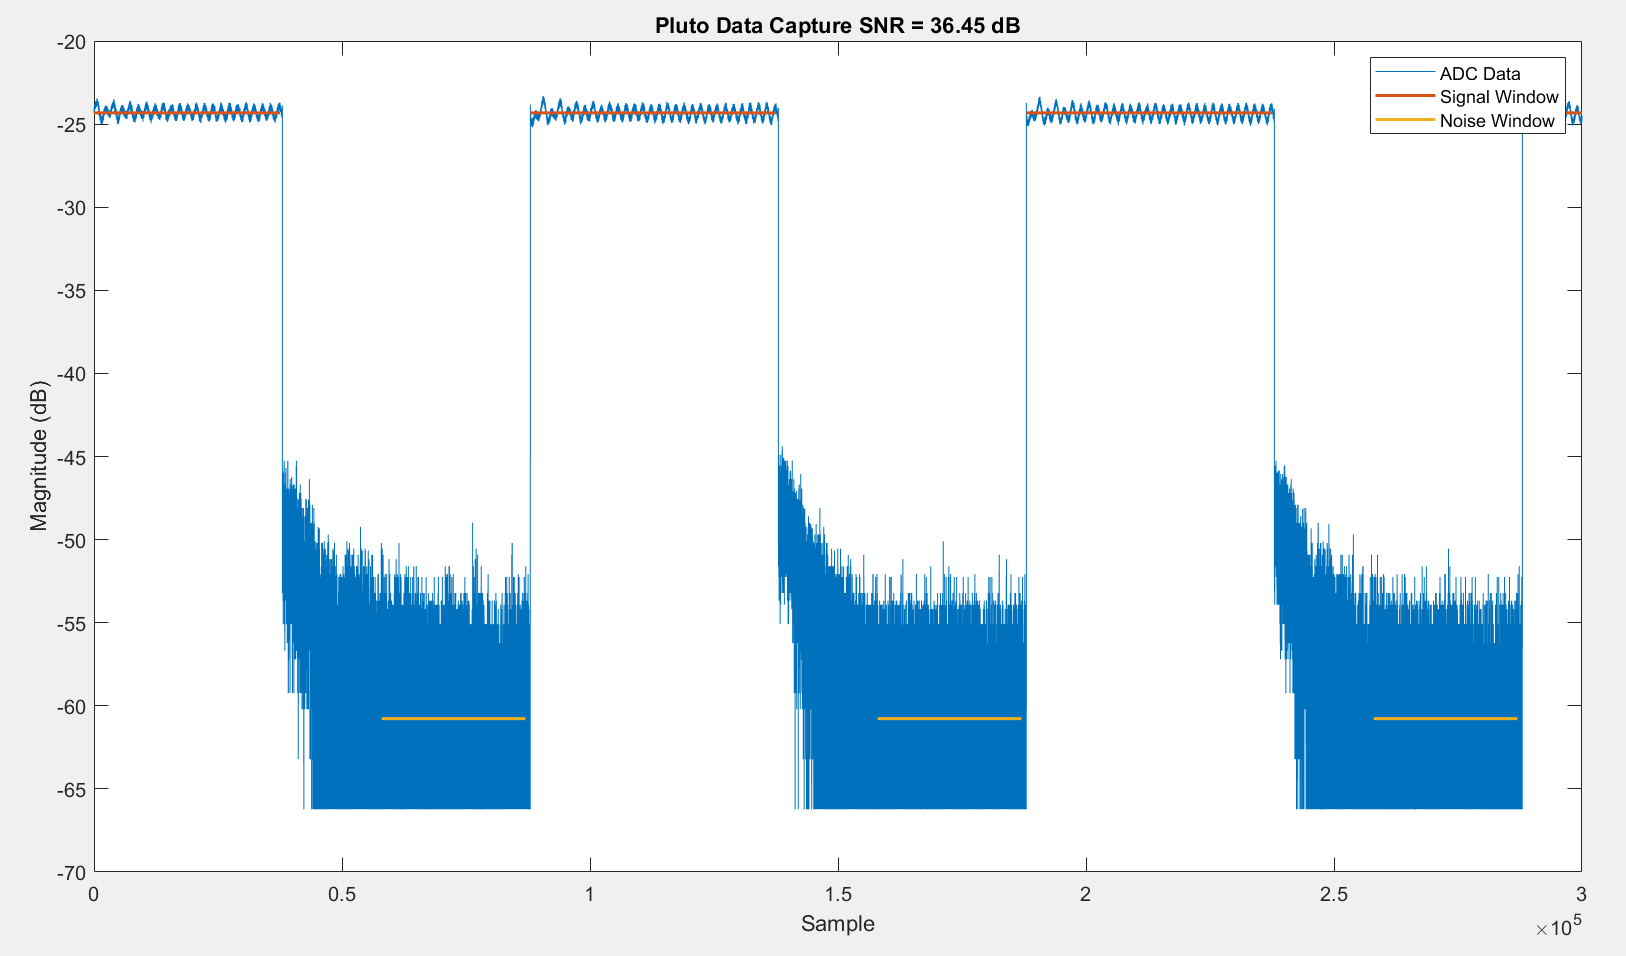
\includegraphics[width=0.6\textwidth]{snr_manual_agc_50db_rx_gain_70db_tx_atten.png}}}
	\caption{Signal Power with 50 dB RX Gain and -70 dB of TX Gain}
	\label{fig::snr_manual_agc_50db_rx_gain_70db_tx_atten}
\end{figure}

Examining the figure, we find that the received SNR is 36.45 dB. For comparison, we also measure the SNR when the transmit signal gain is increased to -50 dB. The resulting signal power is shown in Figure \ref{fig::snr_manual_agc_50db_rx_gain_50db_tx_atten}. Based on the figure, we conclude that the updated SNR is 55.89 dB. This is roughly 20 dB higher than what we previously measured. This occurs because the received signal power increases by 20 dB, while the noise power remains the same.

\begin{figure}[H]
	\centerline{\fbox{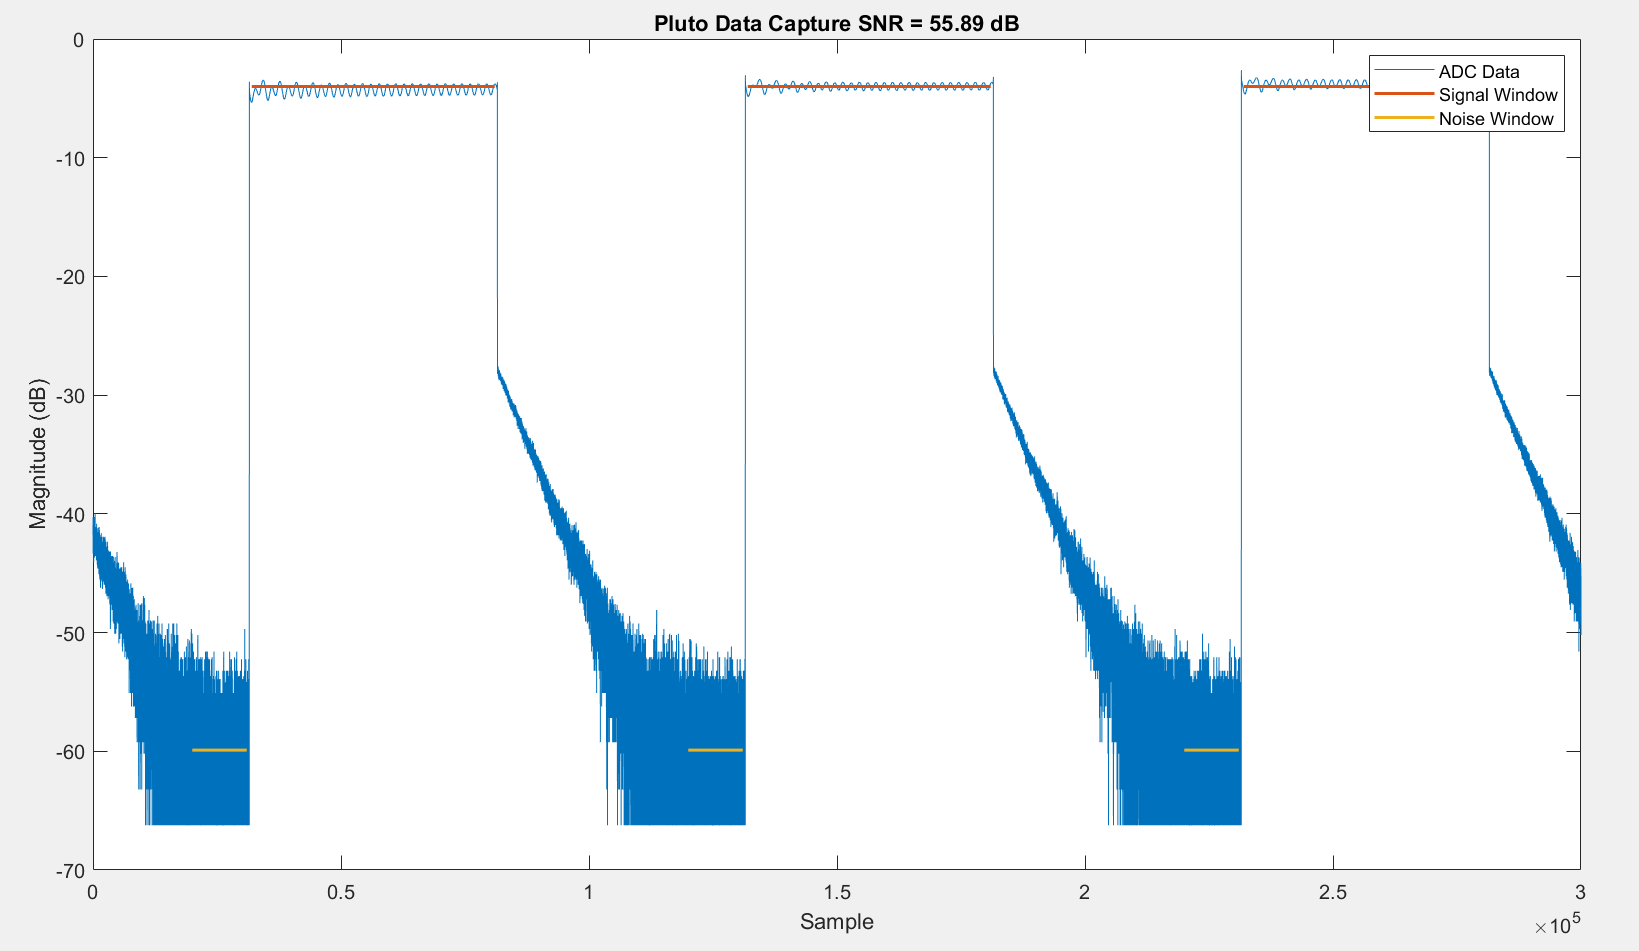
\includegraphics[width=0.6\textwidth]{snr_manual_agc_50db_rx_gain_50db_tx_atten.png}}}
	\caption{Signal Power with 50 dB RX Gain and -50 dB of TX Gain}
	\label{fig::snr_manual_agc_50db_rx_gain_50db_tx_atten}
\end{figure}

We perform a similar experiment by modifying the receive gain while keeping the transmit gain constant. In this experiment, we set the receive gain to 70 dB, while keeping the TX gain at -70 dB. The resulting signal power is shown in Figure \ref{fig::snr_manual_agc_70db_rx_gain_70db_tx_atten}.

\begin{figure}[H]
	\centerline{\fbox{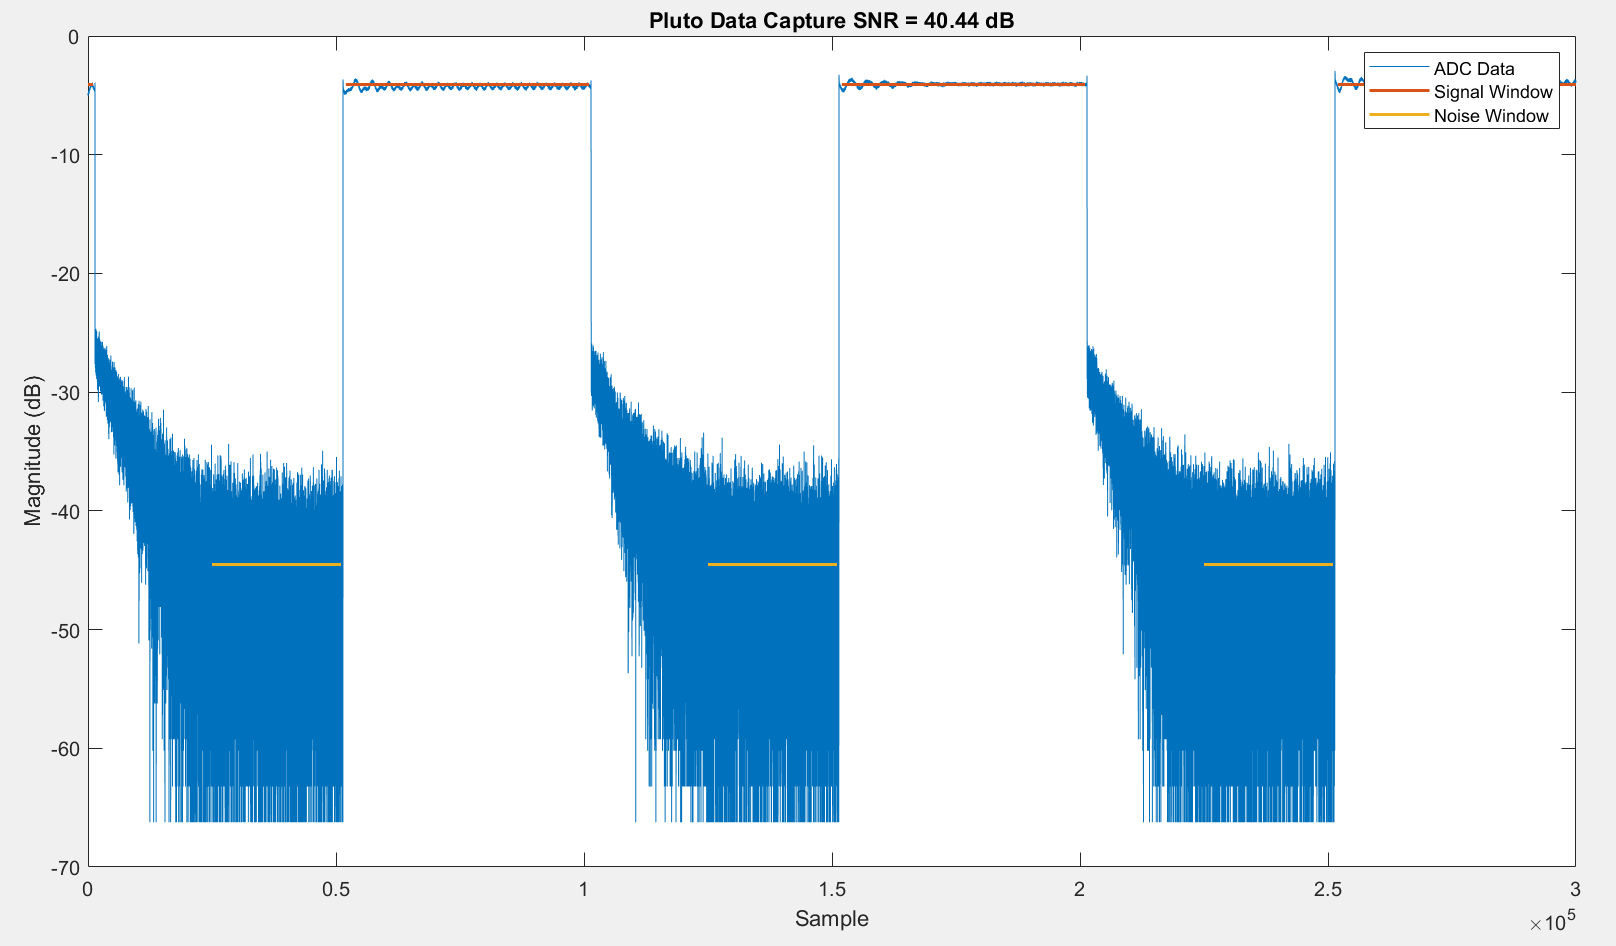
\includegraphics[width=0.6\textwidth]{snr_manual_agc_70db_rx_gain_70db_tx_atten.png}}}
	\caption{Signal Power with 70 dB RX Gain and -70 dB of TX Gain}
	\label{fig::snr_manual_agc_70db_rx_gain_70db_tx_atten}
\end{figure}

Examining the figure, we see that the SNR increases from 36.45 dB to 40.44 dB. What causes the SNR to change when the transmit signal power is constant? The SNR of the received signal is degraded by the noise figure. According to Friss' formula, the noise figure is smallest when the gain in the first gain stage is largest. When the receive gain is increased to 70 dB, the gain in the first gain stage increases, resulting in an SNR increase.

We compare the SNR of the \textit{Manual} AGC data to the SNR when the \textit{AGC Slow Attack} and \textit{AGC Fast Attack} algorithm are used. Figure \ref{fig::snr_agc_slow_attack_30db_tx_atten} shows the instantaneous power when the AGC algorithm is set to \textit{AGC Slow Attack}, and Figure \ref{fig::snr_agc_fast_attack_30db_tx_atten} shows the instantaneous power when the AGC algorithm is set to \textit{AGC Fast Attack}.

\begin{figure}[H]
	\centerline{\fbox{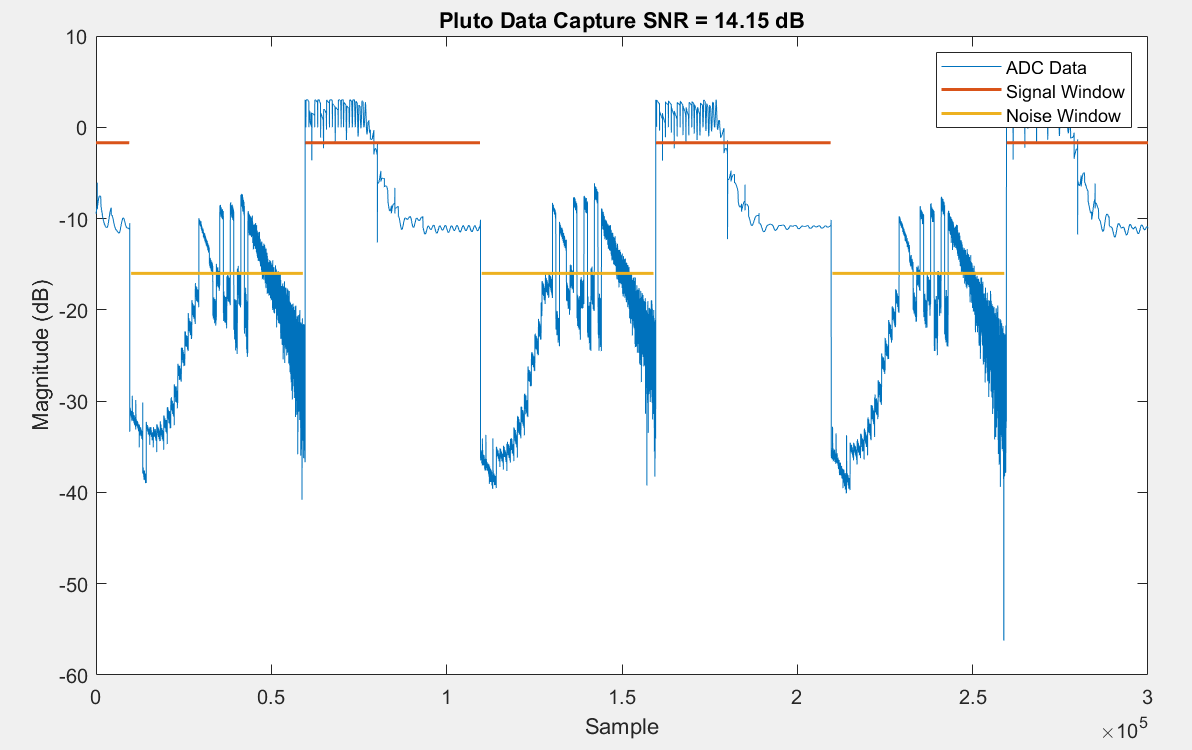
\includegraphics[width=0.6\textwidth]{snr_agc_slow_attack_30db_tx_atten.png}}}
	\caption{Signal Power Measurement with \textit{AGC Slow Attack}}
	\label{fig::snr_agc_slow_attack_30db_tx_atten}
\end{figure}

\begin{figure}[H]
	\centerline{\fbox{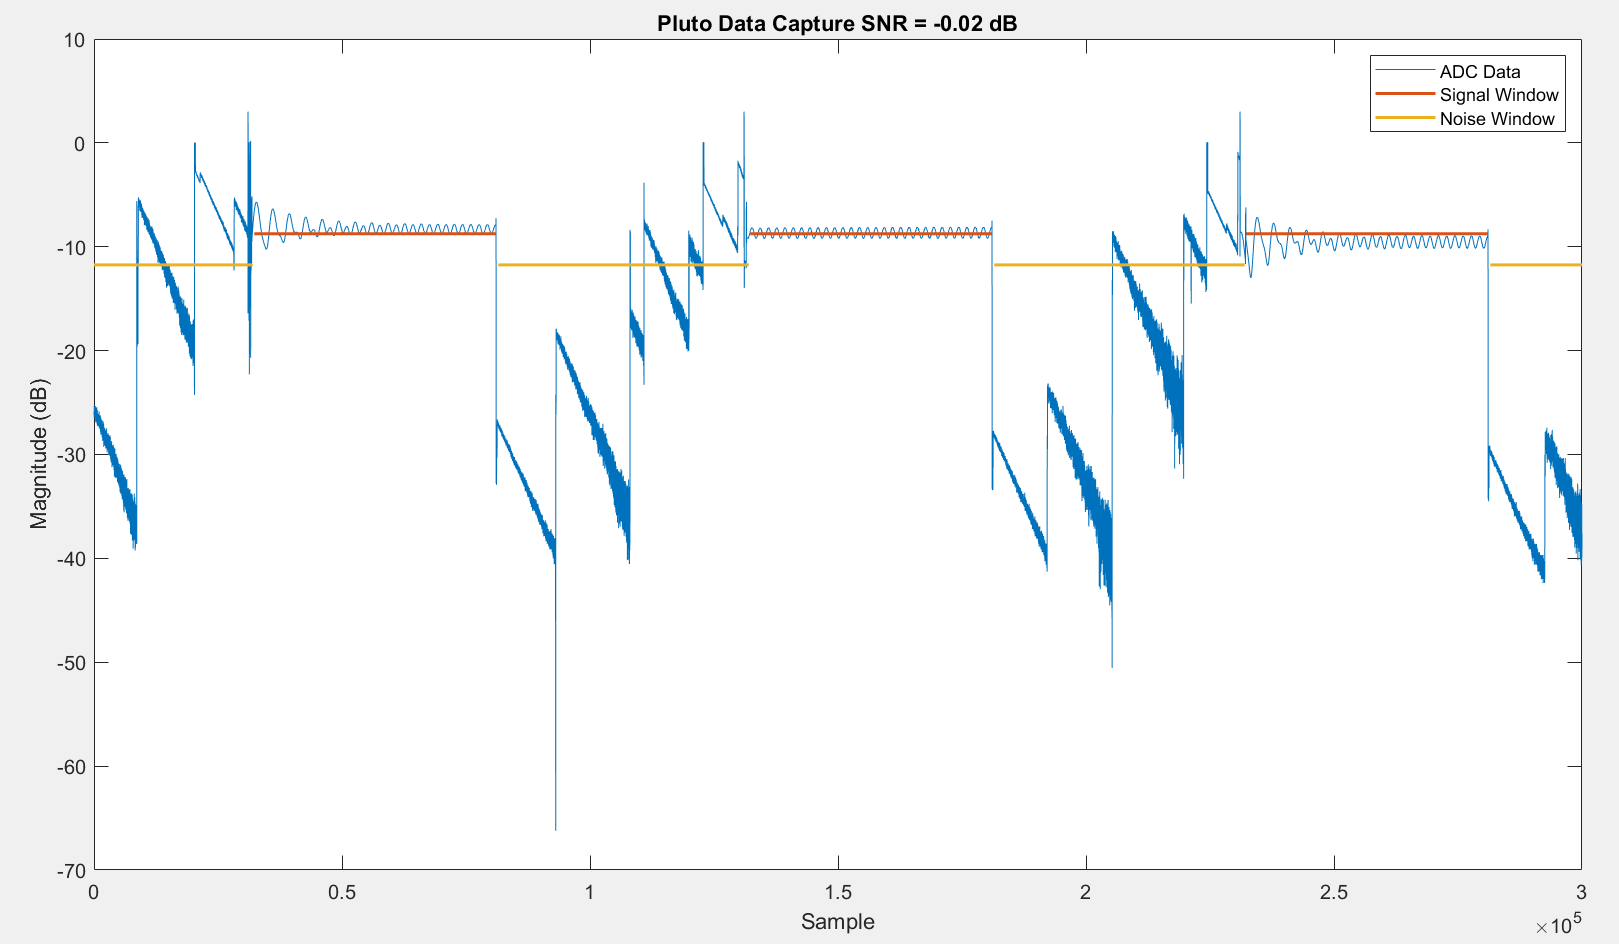
\includegraphics[width=0.6\textwidth]{snr_agc_fast_attack_30db_tx_atten.png}}}
	\caption{Signal Power Measurement with \textit{AGC Fast Attack}}
	\label{fig::snr_agc_fast_attack_30db_tx_atten}
\end{figure}

Examining the above figures, we see that the instantaneous power plots are distorted by both AGC algorithms. The AGC algorithms increase the power of the noise samples to maintain a given headroom. In doing so, they distort our SNR measurement, which depends on constant noise levels throughout the collect. Using the methods mentioned previously, we measure an SNR of 14.15 dB for the \textit{AGC Slow Attack} algorithm and an SNR of -0.02 dB for the \textit{AGC Fast Attack} algorithm. Over portions of the pulse that captured the sinusoid with good AGC settings, the SNR is likely similar to what was measured before. If we took a short-time Fourier Transform (STFT) over these samples, we could use the power of different FFT bins to measure the noise floor and signal power, which would in turn result in a much better SNR estimate. 

\section{Conclusion}
% Conclusions to the overall lab that discuss meaningful lessons learned and other takeaways from the assignment. (Important)

In this lab, we started working with the ADALM-PLUTO Active Learning Module (PlutoSDR). We learned how to interface with the \textit{ad9361-phy} device on the PlutoSDR via IIO. The \textit{ad9361-phy} device in turn controlled the physical layer of the device, applying the transmitter and receiver configurations. After learning about IIO, we performed loopback collects in MATLAB and GNU radio. In MATLAB, we measured the levels of receiver gain, which led to saturation. We then experimented with the \textit{AGC Fast Attack} and \textit{AGC Slow Attack} algorithms. We saw that the \textit{AGC Fast Attack} algorithm responded faster to rapidly changing inputs. However, when exposed to dynamic inputs, both AGC algorithms resulted in distortion (transients and/or clipping).

Next, we performed a loopback collect in GNU Radio. The built-in Pluto Sink and Source blocks provided access to critical device settings which included the RF bandwidth, the cyclic option, and the gain control mode. The RF bandwidth is the bandwidth of the analog filters in the transmitter and receiver. Having too large of an RF bandwidth can lead to an SNR degradation due to extra noise aliasing into our spectrum. The cyclic option allows us to repeat a single buffer of samples in the transmitter. Using the cyclic option allows us to achieve a continuous transmitted data stream, while freeing up USB bandwidth. The AGC settings in the GNU Radio block provide access to all the AGC settings available in MATLAB and an additional hybrid AGC setting. 

In GNU Radio, we also used the provided flowchart to measure the receiver gain that resulted in saturation. When we replaced the QT Time and QT Frequency Sink with the QT GUI Sink, we were given an additional averaging option. This option averaged the power of the FFT outputs resulting in a reduced noise variance and a better estimate of the signal's frequency response. We also collected the frequency response with a rectangular window instead of a Blackmann-Harris window. This change resulted in a reduced mainlobe width at the cost of increased sidelobe levels.

Then, we replaced the PlutoSDR Sink and Source block with equivalent generic IIO blocks. This gave us an opportunity to learn more about the IIO control of the \textit{ad9361-phy}. To validate our work, we repeated the GNU Radio loopback experiment using the updated flowchart. We also updated the LO frequency and sampling rate in the flowchart. Then, we validated that these parameters were correctly applied using the \texttt{iio\_attr} command.

Finally, we used MATLAB loopback collects to measure the SNR of the signal. With \textit{Manual} AGC, our SNR increased linearly as we increased the transmitted signal power. We also observed an SNR gain for fixed transmit powers when we increased the receiver gain. This occurred due to Friss' formula, which states that the noise figure decreases when we apply our gain early in a cascade of amplifiers. We also tried measuring the SNR with \textit{AGC Slow Attack} and \textit{AGC Fast Attack} enabled. These AGC algorithms increased the power of the noise outside of the transmitted pulse, leading to artificial reductions in our measured SNR.

\nocite{analog_devices_libiio_error}
\bibliographystyle{IEEEtran}
\bibliography{sources}{}
%\bibliographystyle{ieeetr}
	
\end{document}